\chapter{Program Architecture}

\label{ch:program}

\newcommand{\term}[1] {{\spaceskip=.95\fontdimen2\font minus \fontdimen4\font
	\xspaceskip=0pt\relax \large\texttt{#1}}}

\renewcommand{\inlinecode}[1]{\colorbox{red}{\lstinline[basicstyle=\ttfamily\color{black}]{#1}}}

\newcommand{\codefunc}[1]{\colorbox{evenmorelightgray}{\lstinline[basicstyle=\ttfamily\color{black}]{#1}}}

\newcommand{\codeobj}[1]{\colorbox{evenmorelightgray}{{\spaceskip=.95\fontdimen2\font minus \fontdimen4\font	\xspaceskip=0pt\relax \large\texttt{#1}}}}

\newcommand{\codeother}[1]{\colorbox{evenmorelightgray}{\lstinline[basicstyle=\ttfamily\color{black}]{#1}}}


\newcommand{\filename}[1] {{\spaceskip=.95\fontdimen2\font minus \fontdimen4\font
		\xspaceskip=0pt\relax \large\texttt{#1}}}


As explained in the introduction (\ref{ch:intro}), the aim of this thesis is to convert a given racing game into an environment that can be played by reinforcement learning agents and to analyze the performance of different agents. In this chapter, I will explain the implementation that was developed throughout this process. I will start by explaining the design decisions that shaped this implementation in section~\ref{ch:projectcharacteristicschap}. In the following section (\ref{ch:implementation}) I will explain the particular source code. I will start with the game as it was given as starting point, most parts of which are not implemented by the author of this thesis. Then the implemented extensions of the game are explained, before leading over to the agent. In the last section of this chapter (section~\ref{ch:possiblefeatures}), I will explain what kind of data the game provides that can be used by an agent.

\section{Characteristics and design decisions}

\label{ch:projectcharacteristicschap}

As stated in chapter~\ref{ch:rlframeworks}, the usual framework for solving reinforcement learning tasks is fairly rigid. However, the task of this work differed in some respects from the usual implementation of a reinforcement learning agent, which led to the necessity of differing from the usual framework in numerous situations. In the following sections, I will provide an overview of the difference between this project and other work in the reinforcement learning domain. Furthermore, I will discuss some of the design decisions that found their way into the final version of the program as well as challenges that occured during its implementation and their respective solution. For that, I will explain general principles in the first section of this chapter, and go into detail about some of the specific details about the implementation in the subsequent section.

\subsection{Characteristics of this project} \label{ch:projectcharacteristics}

There are several differences from this project to others in the reinforcement learning community. The most important difference to the agents presented in chapter~\ref{ch:RL} is, that those are developed as general-purpose problem solvers, with the intention to solve any arbitrary task given to them. In this approach, that is not the case -- the goal is to solve the specific, given game. This allows in principle to incorporate expert knowledge of the task domain, to for example forbid certain combinations of the output or to use particular types of exploration, which are specifically useful in this scenario. The game which is supposed to be played is a racing game, which has implications in several domains, for example making the standard $\epsilon$-greedy approach for exploration much worse as in many other domains. Next to that, the game which is supposed to be played is, in contrast to games solved in openAI's gym-environment (\ref{ch:rlframeworks}), live. While the game could in theory be manually paused for every RL step, it is worth trying to let the agent run ``live'', such that it runs fluently and its progress can manually be inspected. Another challenge was the fact, that the game is coded in a programming language for which no efficient deep learning architectures exist, which led to the necessity of a propietary communication between the environment and its agent.

The fact that there is a game that is supposed to be \textit{solved} also extended the entire problem domain: While usually the focus of developing RL agents can lie purely on the agent, assuming that the environment and consequently its definition of state/observation and reward is fixed, the focus of this work was to learn this one game as well as possible -- in other words it is also necessary to test what a useful definition of observation or reward looks like. Many of the subsequent design decisions are made with the idea in mind, that it must be as easy as possible to compare different agents using a unique combination of state-definition, reward-definition, model and exploration technique. 

Furthermore, the question of how important supervised pretraining is will be addressed in this thesis. For that, the game must provide a way of recording manual actions and their corresponding observation and to record that in a way, that a learner can read it and train on this data. The natural questions arising are how good an agent relying purely on supervised training performs in comparison to others. Another important question is if there is a way to combine pre-training with reinforcement training in racing tasks, as famously done in the board game Go\cite{silver_mastering_2016}.

%differences from mine to others with their implications
%-geht nur um 1 spiel 
%	-settozero sinnvoll (expert knowledge)
%	-andere exploration möglich
%-spiel ist live (nochmal im diagramm zeigen)
%	-dass das härter für den agent ist/er schneller ist
%	-humanTakingControl möglich, man kann sich Q-werte/rewards/.. in situationen angucken
%-verschiedene sprachen
%	-proprietäre kommunikation
%	-spiel ändert sich ebenfalls, was anderes als proprietär wäre dumm
%-human taking control ("wie sind die q-werte vor der wand",..)
%-geht um ein RENNspiel 
%	-epsilon-greedy sucks
%	-sieht tendenziell viel mehr den anfang
%- dieses EINE spiel soll möglichst gut gelernt werden
%	-geht ebenfalls darum was für vektoren sinnvoll sind (freier als torcs)
%	-geht ebenfalls darum was für reward definitionen sinnvoll sind
%	-wie viel FPS er hbaen muss
%	-agent ist für resetten verantwortlich
%	-state und reward gehen nicht fix an python, sondern agent sucht aus
%		-sowas wie annealing reward möglich
%		-man könnte sogar den reward selbst lernen lassen anhand von "mit welcher reward-funktion minimiert er nach 2millionen iterationen die rundenzeit am besten"
%	-Pretraining möglich, vergleichbarkeit mit pretraining, kombination
%
%
%Dinge die also verglichen werden
%	-reward
%	-inputs
%	-model
%	-was den state beendet
%	-exploration techniques
%	-pretraining ja/nein


\subsection{Characteristics of the game}

%at the end of this section a clear distinction between agent and environment should be known. Where does the agent stop, where does the environment begin. 

%-3 actions as input (and braking is necessary)
%-no opponents
%-realistic physics
%-slip
%-dass throttle und brake nur torques applien, was halt realistisch ist, thanks unity
%-indeterministic
%-partially observable
%-huge, non-tabular solvable, continuous state space
%-of course, at best, contiuous action space
%-goal is to finish 1 round in as short time as possible, while staying on track
%-der agent ended mit den actions - das auto ist teil der environment
%-track consists of track, off-track and curb with different friction properties

The given game is a simple but realistic racing simulation. As of now, it consists of one car driving one track. While it possible to implement additional AI drivers or different tracks, no such thing is considered in the current implementation. The main focus of the given simulation lies on realistics physics, which make the game far harder to predict and masterthan many of those implemented for the \term{Atari}-console, on which the original \term{DQN} was tested.

The input expected from an agent consists of three continuous actions: The \keyword{throttle} increases the simulated motor-torque, which leads faster rotation of the tires and thus applying forward force to the car. The \keyword{brake} simulates a continuous brake force slowing down the rotation of the tires. It is not possible to complete a lap while constantly accelerating as much as possible without braking. It is important to note that slip and spin is also simulated: While the rotation of the tires can be accelerated or decelerated fairly abrupt due to their small mass, the car itself has a higher mass and thus more intertia, with forbids abrupt changes in movement. As the tires are rigidly attached to the car, they lose grip on the street, which lessens the impact of consequent forces applied to the tires. The last command an agent must output is the \keyword{steering}, which turns the front tires of the car, leading the car applying force to the respective side the tires steered towards.

It is the task of an agent to provide commands for the values of throttle, brake and steering, which are continous in their respective domains: $throttle \in [0,1]$, $brake \in [0,1]$ and $steer \in[-1,1]$. Of course, as is the general case in reinforcement learning problems, the agent does not know the implications of its actions in advance but must learn them via trial and error. It should however also be kept in mind that the agent provides those actions \textit{to the car}, and that the car must be seen as part of the environment as well, as the actions do not have a reliable impact on its behaviour. For instance, if the car is moving at fast paces, hitting the brake will not lead to an abrupt stop, as the car's inertia still applies a forward force. %wenn considered zu lang, diesen satz mit nem späterem verbinden "In fact, the situation is even worse, as braking at high speeds leads to the effect that the car slips and 
Also, the impact of the steering changes with the movement of the car. For example, the turning circle of the car has a much slower radius in smaller speeds. Another consequence of the realism of the physics implemented in this simulation is the fact that simultaneous braking and steering at high velocities has almost no effect: Because of the high speed, the car has a strong forward force. That leads in combination with the braking to the front tires slipping a lot, which reduces the impact on forces applied to them on the car -- it will not follow the direction of the steering but continue its forward pace determined by the stronger force, namely the inertia.

The track itself is a circular course with a combination of unique curves, requiring the car to steer left as well as right. Along every point of the course, there are three different surfaces providing different friction -- the \textit{track} (inside) itself provides the most grip, while the \textit{off-track} (outside) surface is far more slippery. Between the track-surface and the off-track-surface there is the \textit{curb}, which manifests as a small bump with separate friction properties. The track, curb and off-track each have a consistent width throughout the circuit. To the outside of the off-track there is a wall that cannot be traversed.

\subsubsection{The game as a reinforcement learning problem}

As detailed in chapter~\ref{ch:RL}, reinforcement learning agents are solvers for (possibly only partially observed) Markov Decision Processes with unknown transition relations. In other words, for the agent to successfully learn how to operate in an unknown environment, this environment must correspond precisely to a tuple of $\langle S, A, P, R, \gamma \rangle$ (details explained in section \ref{ch:mdps}). Because in this simulation only the case of a single agent without any other cars on the track is considered, the racing problem can be formalized as a Markov Decision Processes with a similar reasoning than \citet[chapter 4]{wymann_torcs_2000} put forward for \term{TORCS}. As is the general case in simulations, while every update-step of the physics aims to simulate a continous process, those updates must be discretized in the temporal domain. As however both agent and environment run live, the temporal discretization of the agent can not always correspond to that of the environment if an update-step in the agent takes longer than in the environment. To put that into numbers, the fixed timestep for the environment's physics is at 500 updates per second, while the agent discretizes to maximally 20 actions per second.

As mentioned in the previous section, the action space required by the agent is continuous with $\mathcal{A} \subset \mathds{R}^3$. 

The environment's state is a linear combination of different factors, as for example the car's speed, absolute position, current slip-values and much more. While certainly finite, it consists of many high-dimensional values: $\mathcal{S}_e \subset \mathds{R}^{n \in \mathds{N}}$. Because of certain factors in the implementation of the environment itself, the environment is indeterministic\footnote{The game is programmed in Unity, which has non-predictable physics. As discussed for example in \url{https://forum.unity3d.com/threads/is-unity-physics-is-deterministic.429778/}, this is because of the fact that any random-number-generator depends on the current system time, which is never fully equal in subsequent trials. Because the calculation of some states can be more complex than others, this effect can snowball even more -- longer calculation in one step leads to later timing of a subsequent update step, which can lead to a whole other trajectory along the state space, even though the start state was equal.}, while the start-state is always equal. As can in principle be argued that the environment's state corresponds to all information stored in the game's section of the computer's RAM, the game trivially fulfills the markov property. As the environment is only a single-agent system, the transition function of the environments can be expressed as a stochastic function of state and action: $\mathcal{S}_e \times \mathcal{A} \rightarrow \mathcal{S}_e$.

There is no formal definition of a reward returned by the environment in the game. While it could in theory be argued that the inverse of the time needed to complete a lap could be taken as the reward, it is obvious that this is infeasible due to many reasons: Finishing one lap takes several seconds, which means there are hundreds of iterations between start state and final state. Next to the obviously arising \keyword{credit assignment problem}, the chance of an agent even getting to the finish line without crashing, is practically zero without rewarding intermediate progress. Instead, it makes sense to give more dense rewards. As mentioned in section~\ref{ch:projectcharacteristics}, the reward also is subject of experiments in the scope of this thesis. For the game to correspond to a proper environment, this reward must be a scalar value depending on state and action.

Though it is in theory possible to implement an agent that takes the entire underlying state of the environment as its input, an approach like that is far from feasible, as this state also contains much information only necessary for rendering the game. Instead, in the chosen approach the agent only receives an $observation$ of the environment's state. 

Summarizing all those factors, it becomes obvious that the given game can clearly be defined in terms of a \keyword{Partially Observed Indeterministic Markov Decision Process}.

It is worth noting, that while the dimensionality of the observation is likely much smaller than the dimensionality of the state, any feasible observation will be high-dimensional or real-valued. The chance for any particular combination of parameters to appear multiple times is vanishingly low, which makes the use of function approximation necessary.

While the notion of \keyword{POMDP}s itself contains no definition of final states, it is necessary to have use those, as they provide hard limit of the horizon in the calculation of Q-values. Another design decision in the course of the implementation of this project was, that the agent itself can define what it wants to see as the end of an episode. It is a matter of testing after how many seconds the agent shall give up on a trial, or if steering into a wall should be viewed as the end of a training episode. Because of that, the environment provides only candidates of what could terminate an episode to the agent, such that the agent can decide to reset the environment or not. \\

The game itself has three different game modes the user can choose between at the start of the game: In the \term{Drive} mode, users can manually drive the car with the computer's keyboard. If the \term{Train AI supervisedly} mode is activated, the car must still be driven manually, while the game exports information about the driving episode that can be used as (pre-) training data for artificial driving agents. The last mode is the \term{Drive AI} mode, where car can be controlled by an agent, as long as the User doesn't actively interfere. A screenshot of the start menu can be found in figure~\ref{fig:overviewshot} in appendix~\ref{AppendixB}. Note that the background of the menu provides a bird-eye view of the track.

\subsection{Characteristics of the agent}
\label{ch:agentchars}

As stated above, it was a design decision to leave as many options open to the agent as possible, such that several agents can each have their own respective definitions of certain features. To summarize from the above chapters, the features unique to every agent are:
\begin{itemize}
	\item The definition of the agent's \keyword{observation-function}, providing its internal state: $s = o(s_e)$
	\item Definition of the \keyword{reward-function}, returning a scalar from state, action and subsequent state: $\mathcal{S}_e \times \mathcal{A} \times \mathcal{S}_e \rightarrow \mathds{R}$
	\item Definition of its internal \keyword{model}, basing on which it calculates its policy
	\item Under which conditions an episode is considered to be terminated 
	\item Definition of the agent's \textit{exploration technique}
	\item If and how the agent relies on pretraining with supervised data	
\end{itemize}
\begin{flushright}
	\scriptsize
	In the following sections, I will refer to the definitions of these functions/options as the \keyword{features} of the agent. In the implementation, there are many possible features, not all of which are actually used by an agent. I will refer to those as \keyword{possible features}. When I talk specifically about the possible observations influencing the observation-function, I refer to those as \keyword{(possible) vectors}. Furthermore, the specific implementation of the agent's memory will be considered a feature. This has however no further consequences as it only differs in some agents in order to save its replay memory more efficiently.
\end{flushright}

It is due to this design decision that the program flow of this project cannot follow the exact same structure than the one put forward in algorithm~\ref{alg:gym}. One big structural difference is for example that the outer loop (line~\ref{algline:gym_episode}) becomes obsolete, as the agent decides under what conditions the environment must be reset. A further advantage of an implementation like this is also, that it can be experimented with rewards that change over time, such that an agent can for example first learn how to move forward, and only later to always stay on track.

Because there are many features in which agents can differ, it makes sense to use the object-oriented programming concept of \term{inheritance} for the different agents. In such an implementation, the main methods common to every agent as well as basic definitions of the features are implemented in a superclass. Particular agents inherit from this class, while overwriting the attributes/functions for the feature in which they differ.\\

\noindent I will go into detail about the implemented features and vectors in a later section after describing the implementation of agent and environment, as the data relies on functions and data specific to this implementation. 


\section{Implementation}

\label{ch:implementation}

The associated programs are, as will be explicitly stated, written by the author of this work as well as its \leonbase, and are licensed under the GNU General Public License (GNU GPLv3). Their source codes can be found digitally on the enclosed CD-ROM as well as online:. Version control of this project relied on \term{GitHub}\footnote{\url{https://github.com/}}, and was split into three repositories: The source code of the actual game written with the game engine \term{Unity 3D} (\textit{BA-rAIce}\footnote{\url{https://github.com/cstenkamp/BA-rAIce}}), the source code of the implementation, written in \term{Python} (\textit{Ba-rAIce-ANN}\footnote{\url{https://github.com/cstenkamp/BA-rAIce-ANN}}), as well as the present text, written in \LaTeX ~ (\textit{BAText}\footnote{\url{https://github.com/cstenkamp/BAText}}). To ease connections between the following descriptions and their correspondenced in the actual source code, footnotes will refer as hyperlink to the files on GitHub (the relative path on the enclosed CD is equal to those on GitHub). In order to ensure that no work after the deadline is considered, it is referred to the signed commits \colorbox{red}{THE, SIGNED, COMMITS}.
%TODO: signed github commit!

The game is programmed using Unity Personal with a free license for students\footnote{\url{https://store.unity.com/products/unity-personal}}. It is tested under version \term{2017.1.0f3}\footnote{As of now, \today, there is a bug in Unity that causes it to crash due to a memory leak if UI components are updated too often (which happens after a few hours of running). Because of that, in the current release of this project, all updates of the Unity UI are disabled in AI-Mode. A bug report to Unity was filed (case \href{https://fogbugz.unity3d.com/default.asp?935432_h1bir10rkmbc658k}{935432}) on \formatdate{27}{7}{2017}, and it was promised that this issue will soon be fixed. Once that is the case, the variable \inlinecode{DEBUG_DISABLEGUI_AIMODE} in \href{https://github.com/cstenkamp/BA-rAIce/blob/ef2dc018f36cd9ad65df90e65d8ab840c822567e/Assets/Scripts/AiInterface.cs\#L12-L13}{BA-rAIce/AiInterface.cs} can be set to \inlinecode{false}.}.
Scripts belonging to the game are coded using the programming language \term{C\#}. The agent was programmed with \term{Python 3.5}, relying on the open-source machine learning library \term{TensorFlow}\cite{abadi_tensorflow:_2015}\footnote{\url{https://www.tensorflow.org/}} in version \term{1.3}. For a listing of all further used python-packages and their versions, it is referred to the \href{https://github.com/cstenkamp/BA-rAIce-ANN/blob/master/requirements.txt}{BA-rAIce-ANN/requirements.txt}-file. 

While the author of this work contributed most of the work to change the given game such that it can be learned and played by a machine, the original version of the game was given in advance, coded by \leon of this work. While it will be explicitly stated what was already given later in this chapter, it is also referred to the respective branch on Github (\textit{Ba-rAIce -- LeonsVersion}\footnote{\url{https://github.com/cstenkamp/BA-rAIce/tree/LeonsVersion}}). The implementation of the agent was however not influenced by any other people than the author of this work.\\

\noindent As already hinted at, the program flow of the implementation differs from that of other implementations. The game, making up the environment, is completely independent of the agent and runs as a separate \keyword{process} on the machine. The agent is written in another programming language and must thus make up a distinct process as well. Because of that, it is necessary that agent and environment communicate over a protocoll that allows inter-process-communication. In this work, it was decided to use \keyword{Sockets} as means of communication. While explained in following section, it is for now important to know that sockets are best implemented as running in a separate \keyword{thread}, where they can send textual information to another socket running in another process.

\subsection{The game as given}
\label{ch:gamedescription}

The program flow of the game is encapsuled by the framework that the \term{Unity 3D} provides: To ease the implemention of games, Unity provides numerous \term{game objects} with pre-implemented properties like friction or gravity, as well as drag-and-drop functionality to add 3D components or cameras to the Graphical User Interface (\textbf{GUI}). Another advantage of Unity is, that it targets many graphics APIs, which takes a lot of work from the programmer to implement an efficient graphics pipeline.

To implement additional behaviour or features not predefined by Unity, it allows for scripts, written in object-oriented \keyword{C\#}. Scripts that are supposed to be used by Unity must provide a class that extends\footnote{In the following sections, I will use the terms \term{extends}, \term{implements}, \term{knows} and \term{has}. When I use those, I mean them in the strict sense in the context of object-oriented programming languages (and the concepts inheritance, interfaces, and references).} its class \inlinecode{MonoBehaviour} or be used by such a one. 
For the file to be instanciated during runtime, it must be specified in Unity's \term{Object Hierarchy}. After staring the program, Unity will create all objects specified in the hierarchy. To enable the possibility of instanciations \term{knowing} each other during runtime, they must provide public variables of the type of the respective subclass of \inlinecode{MonoBehaviour}, which can via drag-and-drop be assigned to the respective future instance specified in the Object Hierachy. \inlinecode{MonoBehaviour} provides a number of functions that are automatically called by Unity at different times during runtime. The most important ones are \inlinecode{void Start()}, called when first instanciating the respective object, as well as \inlinecode{void Update()} and \inlinecode{void FixedUpdate()}, called every Update-step or Physics-update-step, respectively\footnote{Concerning the difference between Update and Fixedupdate: \textbf{Update} is called once per frame, in other words as often as possible. It is generally not used to update physics, as its call frequency depends on the current \textbf{FPS} -- if calculations here take to long, the FPS of the game will decrease. \textbf{FixedUpdate} is called precisely in a fixed interval of game-internal time. If calculations in FixedUpdate are too slow, the progress of the game-internal time is delayed until FixedUpdate catches up. The update-interval of FixedUpdate can be freely chosen and is $0.002$ seconds in the current implementation. If Unity's \inlinecode{Time.timeScale} is set to zero, FixedUpdate() will not be called at all.}. If a subclass of \inlinecode{MonoBehaviour} is attached to a game object, it can provide specific additional functions that are called when specific events occur during runtime -- an example would be \inlinecode{OnCollisionEnter(Collision)}.\\

In the following, I will describe the game in chunks corresponding roughly to an implemented class, to which the footnote in the headline refers. In appendix~\ref{AppendixC}, I also provide an informal table of each class and its important methods. Keep in mind that the structure of this files as well as most of their content is not created by the author of this thesis. Note also, that I will sometimes mention optinal features. As those options are relevant not to a User of the game but to its developers, those options are specified in the code, more precisely in a static class called \inlinecode{Consts} in \term{AiInterface.cs}\footnote{\label{aiint} \url{https://github.com/cstenkamp/BA-rAIce/blob/master/Assets/Scripts/AiInterface.cs}}.

%TODO was hiervon noch übrig ist \noindent It is hard to describe the game in a way that is understandable for somebody who has not seen any of the code before, as many functions depend on each other, sometimes in circular ways. As however there has to be a start somewhere, it may be the case that some concepts are referenced to before they are fully explained. An example for this is the \inlinecode{QuickPause()}-function: This function's purpose is to pause all physics processes of the game, such that other functionalities running in parallel to it get time to catch up with their calculations. Also, for the game to be played by an agent a \inlinecode{ResetCar}-functionality that can be triggered by another piece of code is useful. While it will be referenced to those functions, their purpose may become clear only later in the text. For an informal description of what each specific file does, it is referred to the table in 


\subsubsection{Game modes\footnote{\label{gamescript}\url{https://github.com/cstenkamp/BA-rAIce/blob/master/Assets/Scripts/GameScript.cs}}}

On the surface, the game has three different game modes that can be active: \term{Drive}, \term{Drive AI} and \term{train AI supervisedly}. These are the three modes the User can choose from in the game's main menu (the UI of which can be seen in figure~\ref{fig:overviewshot} in appendix~\ref{AppendixB}). In the actual implementation however, the game mode is handled a bit different. \inlinecode{mode} is a public string-array of the globally known object \inlinecode{Game} (an instanciation of a \term{GameScript}, a subclass of \inlinecode{MonoBehaviour} specified in \term{GameScript.cs}\textsuperscript{\ref{gamescript}}). \inlinecode{mode} contains one or more strings of the following group: \inlinecode{"driving"}, \inlinecode{"menu"}, \inlinecode{"train\_AI"}, \inlinecode{"drive\_AI"} and \inlinecode{"keyboarddriving"}. If the game's main menu is opened, \inlinecode{mode = ["menu"]}, and in all other cases it is a set consisting of \inlinecode{driving} as well as the respectively obvious elements. This implementation is advantagous, because some behaviour needs to be triggered in multiple modes -- the car's movement is for instance calculated if \inlinecode{Game.mode.Contains("driving")}, which is the case in all three of the above mentioned modes. The current implementation also makes it easier to add further behaviour: If for example an AI-agent shall also function to generate supervised data, one can simply add the respective mode in the \term{Gamescript.cs} file.

The functionality for switching the game mode is specified in the \inlinecode{SwitchMode(newMode)} function, found in \term{GameScript.cs}. After setting the respective mode as described above, this function disconnects any connected Sockets and  activates the required cameras for the mode, updates the UI's Display indicating the mode and calls some further initializing functions (\inlinecode{AiInt.StartedAIMode()} or \inlinecode{Rec-StartedSV\_SaveMode()}), if applicable. Because particularly the initialization of the \inlinecode{drive\_AI}-mode involves connecting with an external Socket, it is done in part in a side thread. This means that the main thread does not wait for the initialization to be finished -- because of that, the \inlinecode{StartedAIMode()}-function sets the variable \inlinecode{AiInt.AIMode} to \inlinecode{true} once it is done. Any behaviour that depends on a successful initialization of the can thus simply check for this variable instead.

The object \inlinecode{Game} is responsible for switching the \inlinecode{mode} to \inlinecode{menu} in its \inlinecode{Start()}-method or after the press of the \keystroke{Esc}-button at any time during the runtime of the game. Besides this, its definition in \term{GameScript.cs} also contains the methods \inlinecode{QuickPause(string reason)} and \inlinecode{UnQuickPause(string reason)}. The purpose of QuickPause is to pause all physics processes of the game, such that other functionalities running in parallel to it get time to catch up with their calculations. For that, the \inlinecode{QuickPause(string reason)}-function sets the Game's \inlinecode{Time.timeScale} to zero, which freezes all of Unity's internal physics, as well as stopping future \inlinecode{FixedUpdate()}-calls. Further, this function removes \inlinecode{driving} from \inlinecode{mode}, so that other driving-related functions in \inlinecode{Update()} are also stopped. Lastly, the QuickPause-mode changes the game's GUI to make the difference visible to the User. While the public function \inlinecode{QuickPause()} could in principle be called from every method of the game, it contains functionalities that are (due to design concepts of Unity) not thread safe, meaning that only the main-thread can call them safely. To enable the possibility of asynchronous threads activating the QuickPause-mode, \inlinecode{Game} contains a public variable \inlinecode{shouldQuickpauseReason}. This variable can be set to a value from asynchronous threads, and the \inlinecode{Game} checks every \inlinecode{Update()}-step (guaranteed to be main-thread and to also be called if QuickPause is active) if another side thread requested to invoke this method.
Once the method that originally invoked QuickPause wants the game to continue its normal process, it must call \inlinecode{UnQuickPause(string reason)} (or request for it to be called). However, QuickPause could have been enabled by another method as well, that is not ready for the normal game process yet. To prevent such a scenario, the methods to start and to end QuickPause must both be called with a string \inlinecode{reason}. In every call of \inlinecode{QuickPause(string reason)}, the function pushes \inlinecode{reason} on \inlinecode{Game}'s List \inlinecode{FreezeReasons}, and in every call of \inlinecode{UnQuickPause(string reason)}, it removes the respective reason from the list and only continues the normal game process if the list becomes empty.

\subsubsection{User Interface\footnote{\url{https://github.com/cstenkamp/BA-rAIce/blob/master/Assets/Scripts/UIScript.cs}}}

The job of the Game's \inlinecode{UI} (an instance of type UIScript) is to update the user interface. This UI is overlayed over the current scene, such that its components can be seen simultaneously to the image of an active camera. In its \inlinecode{MenuOverLayHandling()}-Method, \inlinecode{UI} specifies the view of the game's menu-mode (as can be seen in figure~\ref{fig:overviewshot} in appendix~\ref{AppendixB}), as well as the key bindings to activate the required mode. In the method \inlinecode{DrivingOverlayHandling()}, it sets visibility, content, color or position of numerous UI components (defined in Unitys Object Hierachy), that are seen in non-menu-modes. Both \inlinecode{DrivingOverlayHandling()} and \inlinecode{MenuOverLayHandling()} are called every \inlinecode{Update()}, such that the view elements are always contemporary. Further, the \inlinecode{UI} specifies the \inlinecode{void onGUI()}-function, which Unity calls every time it re-renders the GUI. This function overlays Debug information on the screen and changes the view if the QuickPause-mode is activated.\\

\noindent The User Interface of the game while driving can be seen in the figures~\ref{fig:humandriveshot} and~\ref{fig:aidriveshot} in appendix~\ref{AppendixB}, which are screenshots for the \inlinecode{keyboarddriving} and \inlinecode{drive_AI} mode, respectively. The latter of those screenshots is annotated with labelled boxes around each UI component, with page~\pageref{fig:aidriveshot} explaining each component a bit further\footnote{Note that the entire UI, besides the content behind labels \textbf{A}, \textbf{F}, \textbf{H} and \textbf{I}, was already implemented like this by \leon.}.

\subsubsection{Controls}

If \inlinecode{Game.mode.Contains("keyboarddriving")}, the game is steered with the arrow keys \keystroke{$\leftarrow$} and \mbox{\keystroke{$\rightarrow$}.} The throttle is triggered via the \keystroke{A}-key, whereas the brake is called via \keystroke{Y}. The \keystroke{R} - key flips the reverse gear. Note that as long as the \inlinecode{pedalType} in \term{CarController} is set to \inlinecode{digital}, throttle and brake are binary when controlled via keyboard. 

If \inlinecode{Game.mode.Contains("drive\_AI")} the car is usually controlled by the agent. It is however possible to re-gain control over it via pressing the \keystroke{H}-key. Once that occurs, the variable \inlinecode{AiInt.HumanTakingControl} is set to true, indicating the program that keyboard-inputs must be accepted. This is useful for example if one wants to check if rewards or Q-values are realistic. If human interference of the \inlinecode{drive\_AI} mode is active, it is possible to simulate speeds to the agent (meaning that not the actual speed of the car, but a specified value is sent to the agent). This can be done with the number keys, where the pretended speed is evenly spread between $0~ kph$ (\keystroke{0}) and $250~ kph$ (\keystroke{9}). The \keystroke{P} key is reserved to simulate a full throttle value. To hand control back to the agent, \keystroke{H} must be pressed again. 

In the \inlinecode{drive\_AI}-mode, a user can also manually disconnect or attempt a connection-trial with an agent. The keys to do that are \keystroke{D} and \keystroke{C}, respectively. During any \inlinecode{mode} containing \inlinecode{driving}, \keystroke{Q} can be pressed to activate the \term{QuickPause}-mode, which allows to spectate the current screen. QuickPause is ended with another hit of \keystroke{Q}. 

\subsubsection{The car\footnote{\url{https://github.com/cstenkamp/BA-rAIce/blob/master/Assets/Scripts/CarController.cs}}}

The \inlinecode{car} itself is a \inlinecode{Rigidbody}, which is a Unity-gameObject with certain properties like spatial expanse, mass and gravity. Attached to the \inlinecode{car} is, next to no further mentioned visible components, a Unity \inlinecode{BoxCollider} as well as four \inlinecode{WheelColliders} gameObjects. While the \inlinecode{BoxCollider}'s purpose is to trigger the call of particular functions in scripts attached to other gameObjects upon simulated physical contact, the \inlinecode{WheelColliders} are predefined with certain physical properties, allowing for precise simulation of the behaviour of actual tires. How the car moves is specified in an instance of the class CarController, which is attached to the respective Rigidbody.

All functions of the \inlinecode{CarController} are only called in modes containing \inlinecode{driving}. In its \inlinecode{FixedUpdate()}-step, the script adjusts the wheelCollider's friction according to the current surface the wheels are on, and it is checked if the car moved outside the street's surface. Furthermore the car's velocity as well as some other values are calculated. Finally, the torques for acceleration and braking are applied and the front wheels are turned according to the steering-value. The amount of those torques and angles depend on three values: $steeringValue \in [-1,1]$, $throttlePedalValue \in [0,1]$ and $brakePedalValue \in [0,1]$. If \inlinecode{Game.mode.Contains("keyboarddriving")} or \inlinecode{AiInt.HumanTakingControl == true}, those values depend on the User's keyboard input. Otherwise, if \inlinecode{AiInt.AIMode} is enabled, the values are defined as \term{know}n values from the \inlinecode{AiInt}, namely \inlinecode{nn\_steer}, \inlinecode{nn\_throttle} and \inlinecode{nn_throttle}.

In \inlinecode{CarController.Update()}, the outer appearance of the car is updated, consisting of wheel height, wheel rotation and wheel rotation.

As explained in section~\ref{ch:agentchars}, a connected agent must be able to reset the car at any time during runtime. To allow for that, the \inlinecode{CarController} provides a \inlinecode{ResetCar} method. Additionally, there is a \inlinecode{ResetToPosition}-function that resets the \inlinecode{car} to any specified position and rotation. Because the car must stand still after a reset, it is necessary to completely kill its inertia. To do so, it is not enough to apply zero motorTorque and infinite brakeTorque to the car and call \inlinecode{car.ResetInertiaTensor()} inside \inlinecode{ResetToPosition}, because those values would simply be overwritten in the next call of \inlinecode{FixedUpdate()}. This is why in the given implementation the function \inlinecode{ResetToPosition} sets a boolean variable \inlinecode{justrespawned} to \inlinecode{true}. In every call of \inlinecode{CarController.FixedUpdate()}, it is checked if the car did just reset, and performs the necessary forces to remove all of the car's inertia right there, before setting \inlinecode{justrespawned = false}.


% TODO hier wallcolliderscript

\subsubsection{Position tracking\footnote{\url{https://github.com/cstenkamp/BA-rAIce/blob/master/Assets/Scripts/PositionTracking.cs}}}

To successfully learn useful driving policies, the agent must get precise knowledge of the car's position which goes beyond its mere coordinates. Additional useful information is for example the car's position in relation to the street, or information about the course of the road ahead of the it. To allow for that, the game incorporates a \inlinecode{TrackingSystem}, which is an instance of the class \inlinecode{PositionTracking}). The \inlinecode{TrackingSystem} knows the gameObject \inlinecode{trackOutline} and converts it to an array of coordinates located regularly along the track, each one respectively located at the middle of the street -- the \inlinecode{Vector3[] anchorVector}. Using this array, much high-level information about the track can be calculated. As almost all of the respective functionality was however not implemented was not implemented by the author of this thesis, a short scetch of how it can be used shall suffice.

To calulate the progress of the car in percent, one needs the total length of the track as well as the distance the car advanced so far. The first of those can be calculated by summing up the distances between a coordinate and its successor. To get the approximate distance the car advanced, one needs iterate through the \inlinecode{anchorVector}-array to find the one closest to the car (which happens in \inlinecode{GetClosestAnchor(Vector3 position)}). The cumulated distance of successive vectors until the one closest to the car corresponds roughly to its progress in percent. 

As every successive coordinate in \inlinecode{anchorVector} is in the middle of the street, one can calculate the direction of the street at position \inlinecode{p} by calculating the vector \inlinecode{anchorVector[GetClosestAnchor(p)+1] - anchorVector[GetClosestAnchor(p)]}. This can be used as basis for many further calculations: For instance, the car's distance to the center of the street can be found via by calculating the norm of the orthogonal projection from the car's coordinate onto this vector. The direction of the car relative to the street can be found by calculating the angle between its \inlinecode{direction}-vector and the previosly explained vector.

Besides defining the \inlinecode{anchorVector}-array and other helper-arrays depending on it in its \inlinecode{Start()}-method, the \term{TrackingSystem} calculates the car's current \inlinecode{progress} at every \inlinecode{Update()}-step and triggers the \inlinecode{UpdateList()}-method of the \inlinecode{RecordingSystem} in regular progress-intervals. Furthermore, the \term{TrackingSystem} provides certain public methods that can be used by an agent, namely \inlinecode{getCarAngle()}, \inlinecode{GetSpeedInDir()} and \inlinecode{GetCenterDist()}, the precise content of which will be explained in a later section.

\subsubsection{Tracking time\footnote{\url{https://github.com/cstenkamp/BA-rAIce/blob/master/Assets/Scripts/Recorder.cs}}}

As visible in the game's screenshots (more precisely annotations \textbf{B}, \textbf{C}, \textbf{P} and \textbf{Q} of Figure~\ref{fig:aidriveshot}), the game displays information about the current laptime, the last laptime as well as the time needed for the fastest lap. Futhermore the game provides a visual feedback basing on the time needed for a specific section of the street in comparison to the time that was needed for this section in the fastest lap so far (annotation \textbf{E}). This is possible because the game records current laptime multiple times throughout the course. As mentioned above, \inlinecode{RecordingSystem.UpdateList()} gets called regularly by the \inlinecode{TrackingSystem}. \inlinecode{RecordingSystem} is an instance of the type \term{Recorder}. It contains three lists of \inlinecode{PointInTime}s, for \inlinecode{thisLap}, \inlinecode{lastLap} and \inlinecode{fastestLap}. A \inlinecode{PointInTime} is a \term{serializable} object (also defined in \term{Recorder.cs}) that contains two floats, for a progress and a corresponding time.

An instance of a separate class, \term{TimingScript} (found in \term{TimingScript.cs}\footnote{\url{https://github.com/cstenkamp/BA-rAIce/blob/master/Assets/Scripts/TimingScript.cs}}) is attached to a permeable Collider right on the start/finish line that functions as trigger. As a subclass of \term{MonoBehaviour}, \term{TimingScript} has a \inlinecode{void OnTriggerExit(Collider other)}, that is invoked as soon as another Collider stops contact with it. As the only movable collider is the car's boxCollider, this method is called as soon as the car starts a lap. A lap is considered valid under two conditions: First, the car needs to pass a second collider (confirmCollider, with its attached \term{ConfirmColliderScript}\footnote{\url{https://github.com/cstenkamp/BA-rAIce/blob/master/Assets/Scripts/ConfirmColliderScript.cs}}), which ensures that the car did in fact drive a complete lap instead of backing up right back on the start/finish line. The second condition for validity is, that at no time all four tires of the car hit left the street's surface.

If a lap is considered valid, the \term{TimingSystem}'s \inlinecode{onTriggerExit}-procedure calls \term{RecordingSystem}'s \inlinecode{Rec.FinishList()}-method. Afterwards and under no restrictions, it prepares the start of a new lap by calling \inlinecode{Rec.StartList()}. Once \term{StartList} is called, the \term{RecordingSystem} creates a new List of \inlinecode{PointInTime}s, to which the \term{TrackingSystem} then regularly adds new tuples of progress and corresponding time. Once FinishList is called, the \term{RecordingSystem} checks if the lap just now is a new record, and saves it on the computer's disk if so. In its methods \inlinecode{GetDelta()} and \inlinecode{GetFeedback()}, which are called every \inlinecode{Update()}-step of the \inlinecode{UI}, it can then compare the time of the currently latest progress with the corresponding time of \inlinecode{fastestLap}. \\

\subsection{The game -- extensions to serve as environment}

The code explained so far is sufficient for the game to work in the \inlinecode{keyboarddriving}-mode. The framework for this mode was working entirely when the author of this thesis received it, as it was implemented by the \leonbase. The major additions implemented in the scope of this thesis that were mentioned so far is the behaviour following game modes other than \inlinecode{keyboarddriving} or \inlinecode{menu}, the \term{QuickPause}-functionality, the mentioned additions to the User Interface, the means to \term{reset} the car as well as the functions \inlinecode{GetCarAngle()} and \inlinecode{GetSpeedInDir()} of the \term{TrackingSystem}, which will be more thoroughly explained lateron.

\subsubsection{The minimap cameras\footnote{\url{https://github.com/cstenkamp/BA-rAIce/blob/master/Assets/Scripts/MiniMapScript.cs}}}
\label{ch:minimap}

The content of the minimap cameras can be seen behind annotations \textbf{H} and \textbf{I} of figure~\ref{fig:aidriveshot}. They are implemented to serve as an exclusive or additional input to agents, in the hope of providing enough information to learn sucessful policies. As can be seen, the minimap cameras provide a bird-eye view of the track ahead of the car, by filming vertically downwards. In contrast to the foreshortened main-camera, the minimap cameras are orthogonal, which means that distances are true to scale, irrespectively of their position. Because the cameras are attached to the \inlinecode{car}'s Rigidbody, they are always in the same position relative to the car. In the current implementation, up to two cameras can be used (it is however possible to disable one or both cameras by setting a corresponding value in the class \inlinecode{Consts} in \term{AiInterface.cs}). When both cameras are active, one of them is mounted further away from the car, such that one provides high accuracy whereas the other provides a greater field of view. If only one camera is enabled, its distance is set for tradeoff of accuracy and field of view. As both cameras must be handled separately, this happens in the \inlinecode{Start()}-method of the \term{Gamescript.cs}, which \term{know}s both cameras.

While a previous implementation of a similar functionality was provided by \leon using a complex and inefficient ray-tracing, in this implementation the minimaps base on Unity \inlinecode{Camera}-objects, which are efficiently calculated on the computer's GPU. Attached to each camera is a respective instance of \term{MiniMapScript}. While ordinarily the content of Unity's cameras is directly rendered to the game's main screen, this script contains methods to convert the image of the camera to a format that can be sent to an agent. That is made possible by the usage of a \inlinecode{RenderTexture} as well as a \inlinecode{Texture2D}, which are created as private objects in \term{MiniMapScript}'s \inlinecode{PrepareVision(int xLen, int yLen)}-method. This method is called form outside and expects as parameter the dimensionality of the produced matrix, which is set in the class \inlinecode{Consts} in \term{AiInterface.cs}. 
% TODO dass das visiondisplay nur if needed prepared wird

Both cameras provide the public function \inlinecode{GetVisionDisplay()}. When this function is called, it sets the above mentioned \inlinecode{RenderTexture} as the camera's \inlinecode{targetTexture}, forces the camera to \inlinecode{Render()} to this texture, and then reads the rendered contents into the specified \inlinecode{Texture2D}. After this process, it must reset the camera's \inlinecode{targetTexture}, such that it renders back to the game's main display, such that it can be inspected visually. The \inlinecode{Texture2D} however can be then be read pixel by pixel and thus converted to an array or string. As it was decided that the resulting display only differentiates between \term{track}, \term{curb} and \term{off}, the cameras use a \inlinecode{Culling Mask} that visually filter out all other gameObjects.

\subsubsection{Recording training data\footnote{\url{https://github.com/cstenkamp/BA-rAIce/blob/master/Assets/Scripts/Recorder.cs}}}

\label{sec:exportdata}

For the game to be played by an AI agent, data of the environment must be recorded in regular intervals, to either be sent to the agent in the case of it playing the game or learning via reinforcement learning, or to be exported to a file, which an agent can perform pretraining on. In the following sections, I will not talk about what those data exactly looks like, but only how it is saved and sent. Because of that, I will refer to this data under the name \term{vectors}, which are in detail explained in section~\ref{ch:thevectors}. Collecting the lastest \term{vectors} happens in the function \inlinecode{GetAllInfos()} of \term{AiInterface.cs}, which calls a number of functions and returns a string containing the combined result of those.

As calculating the data that needs to be exported can take relatively much time, this process cannot be performed every \inlinecode{FixedUpdate()}-step. Because of that, the following function is used to perform a function in regular time intervals:
\begin{lstlisting}[language=C#, style=CSharp, frame=none]
long currtime = AiInterface.UnityTime();
if (currtime - lasttrack >= Consts.trackAllXMS) {
	lasttrack = lasttrack + Consts.trackAllXMS; 
	SVLearnUpdateList ();
}
\end{lstlisting}%

Where \inlinecode{AiInterface.UnityTime()} returns Unity's internal time by calling \inlinecode{Time.time * 1000}. Using this definition of time has the advantage that it is maximally precise inside Unity, as the time of calling \inlinecode{FixedUpdate()} is likewise dependant on \inlinecode{Time.time}. A disadvantage of this measurement of time is however, that it can only be used in the main thread and asynchronous methods must rely on the system's time, for which no conversion method exists.

Once user selects the \term{Train AI supervisedly} mode, Recorder's \inlinecode{void StartedSV\_SaveMode()} gets called, which enables the minimap-cameras and sets \inlinecode{SV\_SaveMode = true}. If that variable is \inlinecode{true}, the recorder will in its \inlinecode{StartList()} create a new \inlinecode{SVLearnLap = new List<TrackingPoint> ()}. \inlinecode{TrackingPoint} itself is a class defined in \term{Recorder.cs}, that contains certain values about the state of the game, if provided at creation. While driving, the recorder checks every \inlinecode{FixedUpdate()}-step with the mentioned method if it calls \inlinecode{SVLearnUpdateList()}. This method then collects the recent values for the currently performed actions, laptime, progress and speed as well as the respectively latest \term{Vectors}, creates a \inlinecode{TrackingPoint} from those and updates the \inlinecode{SVLearnLap} with it. When the RecordingSystem's \inlinecode{FinishList} function is called upon the next crossing of the start/finish line, the \inlinecode{SVLearnLap} is saved to a file. As the vectors can contain multiple pixel matrices from the minimapcameras, this may however take quite long. To prevent the game from freezing everytime the car passes the start/finish line, the saving of the actual file is performed in a seperate thread.

Because the agent using this exported data is written in another programming language than the environment, the data cannot be exported as binary file. In this implementation, it was decided to save the data in the \term{XML}-format. It is worth mentioning that not only the List of \inlinecode{TrackingPoint} is exported, but also additional meta-information, stating among others the interval of how often a \inlinecode{TrackingPoint} was exported, which can be interpreted and used by an agent as well as manually inspected.

\subsubsection{Communicating with an agent\footnote{\url{https://github.com/cstenkamp/BA-rAIce/blob/master/Assets/Scripts/AiInterface.cs}}\textsuperscript{,}\footnote{\url{https://github.com/cstenkamp/BA-rAIce/blob/master/Assets/Scripts/AsyncClient.cs}}}

%TODO to detect if the car hit a wall (which may require an agent to reset the environment), the wall has an attached WallColliderScript, that can notify an agent upon \inlinecode{onCollisionEnter} by sending the message "wallhit" via sockets.

As already mentioned, the game is running live and is in general not stopped by the agent, as done for example when interfacing with the openAI gym (section~\ref{ch:rlframeworks}). Because of that, the speed of communication between agent and environment is a bottleneck in how good an agent can perform, and needs to be as fast and efficiently implemented as possible. To ensure quick reaction times, it was also decided that agent and game must run on the same machine, as sending the data to another machine increases the needed time drastically\footnote{This is the reason this project was implemented entirely under Windows: There is no stable Unity Editor for Linux, and there is no contemporary GPU-supporting TensorFlow under Mac. The only common ground for which both are available ist therefore the Windows platform.}.

In the scope of this thesis, it was experimented a lot with the flow of communication between agent and environment, with the current version as its most efficient one so far. While there are multiple possibilities of how two different programming languages can communicate with each other (for example \textit{zero-mq}, \textit{named pipes} or \textit{shared memory}), it was decided to use \term{Sockets} for the communication. In most use cases, sockets are used to communicate over the internet, which is why they normally abstract data over several layers, before being sent to another machine. When both sockets are on the same machine and communicate over localhost however, the unnecessary layers are skipped, making a connection over sockets very efficient\footnote{As is explained by alleged former Microsoft networking developer Jeff Tucker in this Stackoverflow-thread: \href{http://stackoverflow.com/questions/10872557/how-slow-are-tcp-sockets-compared-to-named-pipes-on-windows-for-localhost-ipc}{http://stackoverflow.com/questions/10872557/how-slow-are-tcp-sockets-compared-to-named-pipes\,-on-windows-for-localhost-ipc}}. Using the current implementation, reaction times with an average of $30ms$ were archived (including the network inference), which is fast enough for all purposes.

Communication over sockets generally asymmetric: There must always be a \term{Server} and one or more \term{Clients}, both of which contain instances of the class \term{Socket}. Upon being started, the server registers a server-socket at a certain \term{Port} of the machine, where it can be found by clients. It is only possible for clients to connect to it as long as the server keeps up this socket, which is why it is advisable to do so in a separate thread. When a client is started, it needs to know the IP-adress of the server (in this case localhost), as well as the number of the port the corresponding socket waits at. Once the client finds a waiting server-socket behind the port, it is common practice that the server creates a new socket at another port. While this new socket represents a stable connection between server and client, the original server-socket can keep on waiting for new clients to connect to in the future. One characteristic when using sockets as means of communication is, that the communicating sockets need to know the length of a message, to know when to stop reading the input stream. To do that, the length of each message will be transmitted with it.

In this project it was decided that the game functions as a client, whereas the server is written in python. This fits the scheme of the implementation, where the main loop happens in python, with the game only considered as an additional thread providing the agent's input (as can be seen in figure~\ref{fig:sequenceserver}).

If the \term{Drive AI} mode was selected in the game's \inlinecode{menu}, the \inlinecode{AiInt} (an instance of the class AiInterface\textsuperscript{\ref{aiint}}) calls 
its function \inlinecode{StartedAIMode()}, which, next to calling the known \inlinecode{PrepareVision} of the cameras, creates two instances of \inlinecode{AsynchronousClient}, a class defined in \term{AsyncClient.cs}\footnote{\url{https://github.com/cstenkamp/BA-rAIce/blob/master/Assets/Scripts/AsyncClient.cs}}

the function \inlinecode{LoadAndSendToPython}.


%TODO - ungefähres UML-diagramm DES SPIELS!!
%-ablaufdiagramm vom server-zeug dass zu dem von python passt
%-Aufbau des exportierten XMLs (dabieschreiben dass action und speed 2 mal drin sind weil die von fake_speed affektiert sein könnten)
%-beschreibung der optionen-konstanten
%-dass bei ResetToPosition das AIInt pyhtoon drauf hinweist

-warum ich senden und empfangen mit nem DIFFERENT socket mache (dann ists in 2 threads und kann asyncrhon sein aka nichta ufgehalten werden)
-dass es entweder raw data oder special commands schickt

-nochmal drauf eingehen dass das spiel live ist
-das von leon gemalte ablaufdiagramm
\colorbox{red}{dass der server alle 0.1 sekunden was von unity bekommt!}
\colorbox{red}{dass der client mitbekommt wenn nen connection delay entsteht und dann 
	Unity automatisch pausiert (deswgen quickpausereason)! mega das feature!!!}


\subsection{The agent\footnote{I will rely heavily on UML sequence diagrams and class diagrams to explain program flow and classes of agents. In case a reader is unfamiliar with the standards of UML 2.0, it is referred to e.g. \url{https://www.ibm.com/developerworks/rational/library/3101.html} for sequence diagrams and \url{https://www.ibm.com/developerworks/rational/library/content/RationalEdge/sep04/bell/index.html} for class diagrams. In the main text, only small class-diagrams accompany the explanation of the code, with respective complete versions in  \colorbox{red}{appendix~\ref{BLABLABLA}.}}}

As already explained, the implementation at hand differs in its program flow from other implementations, as the environment cannot be specified in a separate class, on which the agent can perform a function like \inlinecode{step()} (as in line \ref{algline:gym_envstep} of algorithm~\ref{alg:gym}). As the closest equivalent to such a class, the file  \term{server.py}\footnote{\url{https://github.com/cstenkamp/BA-rAIce-ANN/blob/master/server.py}} (from now on called server) contains the thread-safe class \inlinecode{InputValContainer} that provides explicit functions to read its state. Upon executing the server, an instance \inlinecode{inputval} of type InputValContainer is created. This instance is \term{know}n to objects that read or write from it through \inlinecode{containers}, an instance of the class \inlinecode{Containers}. This class contains references to several objects and settings that must be known to multiple objects and functions, which can thus for example easily access the mentioned input-value as \inlinecode{containers.inputval}.

It is further important to keep in mind, that the server receives \textit{raw data} from the client, and not a tuple consisting of \inlinecode{observation, reward, done}. The raw data is forwarded to the agent, which calculates the respective \textit{features} on its own. The next section will detail how the server initiates threads needed for the communication with the environment, before leading over to the main loop of the learning process.

\subsubsection{Communicating with an environment}

The behaviour that will be explained is represented graphically in the sequence diagram in figure~\ref{fig:sequenceserver}. 

The main loop of the agent is started by the \inlinecode{main}-method of the server. Upon execution of the this file, it interprets any passed arguments and starts the method. %TODO auf die argumente zurückkommen die Übergeben werden
To allow a fast communication with the game, the main loop of the server is multi-threaded, such that a stable socket-connection to Unity can be preserved while the agent performs its actions in another thread. This may lead to some objects being accessed by different threads (like for example \inlinecode{outputval}), which requires a thread-safe implementation of them.

In its \inlinecode{main}-method, the server creates two server-sockets\footnote{More precisely, the server uses a wrapper-class called \inlinecode{MySocket} (defined in \term{server.py}), which provides the additional behaviour of prepending the length of the future message to it, such that the socket on the other end knows how much it needs to read.}, one on the receiver-port (which is equal to Unity's sender-port), and another one on the sender-port (Unity's receiver-port). Afterwards, the server creates an agent of choice by initializing it and calling its \inlinecode{initForDriving}, passing command-line-parameters. Afterwards, the \term{InputValContainer} \inlinecode{inputval} as well as an \term{OutputValContainer} termed \inlinecode{outputval} are created, and their references are added to \inlinecode{containers}. Once those are created, the server starts two \term{thread}s, more precisely a \inlinecode{ReceiverListenerThread} and a \inlinecode{SenderListenerThread}. These threads use their respective server-socket they know through \inlinecode{containers}, and wait on their port by calling the socket's \inlinecode{accept()}-method over and over.

Once a client connects to one of those listener-sockets, a new connected socket is created. Using this socket, a \inlinecode{receiver\_thread} or \inlinecode{sender\_thread} is created respectively, representing a stable connection to Unity. After creating this thread, the ListenerThread lets \inlinecode{containers} know about its reference (by appending it to \inlinecode{containers.receiverthreads} or \inlinecode{containers.senderthreads}) and starts its listening-loop over again. This means that during runtime, the two ListenerThreads are always active. If for some reason the old \inlinecode{receiver\_thread} or \inlinecode{sender\_thread} loses its connection, the ListenerThreads will simply estabish a new one and create a new thread. Both \inlinecode{receiver\_thread} and  \inlinecode{sender\_thread} contain a method to destroy themselves if needed, such that at any time there is exactly one thread responsible for the connection with Unity.

It was experimented with an explicit learn-thread, which runs in parallel to all other threads. As however the very same TensorFlow-model is needed for learning and inference, doing so in parallel emerged to increase the reaction time of the server from about $30ms$ to about $300ms$. While forcing the inference to run on the CPU and the learning to run on GPU decreased the delay a bit, the performance was still far from satisfactory and the idea was dropped.

While the main thread is constantly running, it does not contribute to the agent's process after initializing all threads and objects. Instead it can, if the agent provides methods to fill it, run the mainloop of the GUI (defined in \term{infoscreen.py}\footnote{\url{https://github.com/cstenkamp/BA-rAIce-ANN/blob/master/infoscreen.py}}), which is programmed with the package \term{tkinter} and must be in the main thread. To allow for side threads to write content to the GUI, its respective widgets (\inlinecode{Text} and \inlinecode{Canvas}) are replaced by thread-safe wrapper-classes using \term{queue}s. When a side thread wants it to print information, it appends the new content to the queue, whereas the main thread always pops the latest element from that queue to print it. Side threads know those wrappers over the dictionary \inlinecode{containers.screenwidgets} and can call the \inlinecode{write} or \inlinecode{updateCol}-method of the respective element.

The main-thread listens for a termination of the user with \keystroke{CTRL}+\keystroke{C}. Once that occurs, it notifies all other threads to shut down by setting \inlinecode{containers.KeepRunning = False} and waits for their termination by \inlinecode{join}ing them, such that the main thread is guaranteed to be the last to finish.

% TODO - Why I have inputval and outputval: INPUTval damit der immer nur die letzte action hinzügen muss und der die history DADRIN hat, und OUTPUTval damit das multithreading schneller geht. BEIDES hat  seinen sinn!! 
%TODO [multiple threads deshalb weil das geschwindigkeit optimiert - beim inputval können mehrere agents multi-threaded unabhängig/gleichzeitig lesen und performen (dann gäbs nen weiteren thread, der wäre dann nicht blau und würde auf inputval zugreifen), und beim outputvall können senderthread und receiverthread einfach gleichzeitig so schnell wie möglich arbeiten]

\begin{figure}[h!]
	\centering
	\resizebox{1.1\textwidth}{!}{
		\begin{sequencediagram}[1]
%	\tikzstyle{inststyle}+=[top color=gray!10, bottom color=blue!50, rounded corners=3mm]
	\tikzstyle{inststyle}+=[top color=blue!50, bottom color=blue!50, rounded corners=2mm]
	\newthread{unity}{:Unity.Client}{0}
	
%	\tikzstyle{inststyle}+=[top color=gray!80, bottom color=yellow, rounded corners=0mm] 
	\tikzstyle{inststyle}+=[top color=yellow, bottom color=yellow, rounded corners=0mm] 
	
	\newthread[blue!60][.5]{recthread}{:receiverThread}{15}
	\newinst{recsoc}{rec:MySocket}{0}
	\newinst{inputval}{:InputVal}{0}
	\newinst{agent}{:Agent}{0}
	\newinst{outputval}{:OutputVal}{0}
	\newinst{sendsoc}{send:MySocket}{0}
	\newthread[yellow]{sendthread}{:senderThread}{14}
	\newthread[red]{reclist}{:RecListenThread}{5}
	\newinst{recwaitsoc}{:MySocket}{0}
	\newthread[white]{main}{main:Thread}{0}
	\newinst{sendwaitsoc}{:MySocket}{0}
	\newthread[green]{sendlist}{:SendListenThread}{6}
	
	\begin{messcall}{main}{init()}{agent}{}		
	\end{messcall}		
	\begin{messcall}{main}{init()}{inputval}
	\end{messcall}	
	\begin{messcall}{main}{init()}{outputval}{}		
	\end{messcall}
	\begin{messcall}{main}{init()}{recwaitsoc}{}		
	\end{messcall}		
	\begin{messcall}{main}{init()}{sendwaitsoc}{}		
	\end{messcall}		
	\mess{main}{start}{reclist}
	\mess{main}{start}{sendlist}
	\begin{sdblock}{loop}{client==None}
		\begin{call}[2]{reclist}{accept()}{recwaitsoc}{client}
		\end{call}
	\end{sdblock}
	\prelevel\prelevel\prelevel\prelevel
	\mess[1]{unity}{connect}{recwaitsoc}
	
	\prelevel\prelevel\prelevel\prelevel
	\begin{sdblock}{loop}{client==None}
		\begin{call}[2]{sendlist}{accept()}{sendwaitsoc}{client}
		\end{call}
	\end{sdblock}
	\prelevel\prelevel\prelevel\prelevel
	\mess[1]{unity}{connect}{sendwaitsoc}
	\postlevel\postlevel
	
	\begin{call}{reclist}{init(client)}{recsoc}{recsocket}
	\end{call}			
	\begin{call}{sendlist}{init(client)}{sendsoc}{sendsocket}
	\end{call}				
	\postlevel\postlevel
	\mess[0][sendsocket]{sendlist}{start}{sendthread}
	\mess[0][recsocket]{reclist}{start}{recthread}
	\begin{sdblock}[green!20]{loop}{mainthread does not send stop-message}
		\begin{sdblock}{loop}{data==""}
			\begin{call}[2]{recthread}{myreceive()}{recsoc}{data}
			\end{call}		
		\end{sdblock}	
		\prelevel\prelevel\prelevel\prelevel
		\mess[1][data]{unity}{send}{recsoc}				
		\postlevel\postlevel
		\begin{call}{recthread}{\small handle\_special\_commands(data)}{recthread}{}
			\begin{sdblock}{opt}{data == \textit{special command}}
				\begin{call}{recthread}{read()}{inputval}{result}
				\end{call}
				\begin{messcall}[0]{recthread}{\small endEpisode(result)}{agent}
					\begin{messcall}{agent}{reset()}{inputval}{}
					\end{messcall}
					\begin{messcall}{agent}{reset()}{outputval}{}
					\end{messcall}								
					\begin{messcall}{agent}{send\_via\_thread("reset")}{outputval}{}
						\mess{outputval}{reset}{sendthread}					
					\end{messcall}						
				\end{messcall}
				\begin{messcall}[0]{sendthread}{mysend("reset")}{sendsoc}{}		
					\mess[1]{sendsoc}{reset}{unity}
				\end{messcall}				
				\prelevel
			\end{sdblock}
		\end{call}
		\begin{messcall}{recthread}{update(data)}{inputval}{}
			\begin{call}{inputval}{\scriptsize append(data)}{inputval}{}
			\end{call}				
		\end{messcall}
		\begin{call}{recthread}{read()}{inputval}{content}
		\end{call}
		\begin{messcall}[0]{recthread}{performAction(content)}{agent}{}
			\begin{messcall}{agent}{\small update(action)}{outputval}{}
				\begin{call}{outputval}{\small send\_via\_thread(action)}{outputval}{}
					\mess{outputval}{send}{sendthread}					
				\end{call}					
			\end{messcall}
		\end{messcall}
		\prelevel
		\begin{call}{sendthread}{read()}{outputval}{content}
		\end{call}			
		\begin{messcall}[0]{sendthread}{mysend(content)}{sendsoc}{}		
			\mess[1][content]{sendsoc}{send}{unity}
		\end{messcall}		
		
	\end{sdblock}
	
	\prelevel\prelevel\prelevel\prelevel\prelevel
	\begin{sdblock}{loop}{user does not interfere}
		\begin{call}{main}{updateGUI()}{main}{}
		\end{call}
	\end{sdblock}
	
	\mess{main}{stop}{recthread}
	\mess{main}{stop}{sendthread}
	\mess{main}{stop}{reclist}
	\mess{main}{stop}{sendlist}

\end{sequencediagram}
	}
	\caption{Sequence Diagram of the Server}
	\label{fig:sequenceserver}
	\medskip
	\scriptsize
	Reading instructions: Y-axis is time. Columns with a full colored bar are threads, other objects are objects. The color of a bar represents which thread a method runs in. An arrow from A to B means "A calls a method from B". %TODO Simultaneous things are horizontally aligned. Messages from thread to thread are without parantheses?
\end{figure}

\subsubsection{The main loop}

In the \inlinecode{receiver\_thread}, the socket is constantly waiting for data. When it receives data, it first checks if it was the usual raw data used for the agent's observation/reward or a \textit{special command}. If it was the latter, the receiver\_thread calls the agent's function \inlinecode{handle\_commands} which will, according to its preferences, terminate the episode (for which it resets \inlinecode{inputval} and \inlinecode{outputval} and notifies the environment to reset itself, more on that later). 

If the data was no such command, the \inlinecode{receiver\_thread} updates the \inlinecode{inputval} and starts an inference of the agent by calling its method \inlinecode{performAction}, passing the latest content of the \inlinecode{inputval}. This method is where the agent calculates its observation/reward, adds this to his replay memory, calculates the action on basis of its model and performs learning steps as appropriate. Immeadiately after the action is calculated, the agent updates the \inlinecode{outputval} with the the result. Upon being updated, the outputval informs the \inlinecode{sender\_thread} of this update. This thread can then read the latest \inlinecode{outputval} and send it back to the client using its socket, which may be simultaneous to the agent performing its learning-step\footnote{Note that all of the agent's inference runs thus in the receiver-thread. It was experimented to use an additional agent-thread that in regular intervals looks if the \inlinecode{inputval} was filled with new data, such that the inference of the agent and a waiting to receive new data can occur simulatenously. However, as the agent's inference runs fast enough if it does not perform a learning-step after an inference and too slow in any case if it does, this concept was abandoned.}. 

As mentioned above, the \inlinecode{inputval} is the server's closest correspondance of the environment. Every time new raw data from the game is sent to the server, \inlinecode{inputval.update} is called, which then incorporates the new information as well as timestamps of when they were send (used to calculate how long an inference took). Because the information that is sent over the sockets is textual, the method \inlinecode{cutoutandreturnvectors} from the file \term{read\_supervised.py}\footnote{\url{https://github.com/cstenkamp/BA-rAIce-ANN/blob/master/read_supervised.py}} is called to convert this text back to python-arrays. Note, that there will consistently be made a difference between the content of the minimap-cameras (vision-vector, see \ref{ch:minimap}) and the other \term{vectors}, as they are stored in a different type of object. While the vision-vectors are stored as 2-dimensional \keyword{numpy}-array, the other vectors are bundled to a class called \inlinecode{Otherinputs}, a subclass of  \term{namedtuple}\footnote{\url{https://docs.python.org/2/library/collections.html#collections.namedtuple}}, which provides easily readable dot-access to its members instead of solely by index. This allows to add new vectors easily, as only a name of the new feature must be added in the definition of \inlinecode{Otherinputs} in the file read\_supervised.py. Further, it increases the overseeability of functions using its components a lot.

The \inlinecode{inputval} contains arrays to store the history of vision-vectors (\inlinecode{vvec\_hist}), otherinputs (\inlinecode{otherinput\_hist}) as well as an array for the history of performed actions (\inlinecode{action\_hist}). In its \inlinecode{update}-method, it normalizes the \inlinecode{otherinputs} and appends it as well as the latest vision-vectors, where it merges both into the \inlinecode{vvec\_hist}.
To reduce the computational load, the \inlinecode{inputval} does not contain the entire history of the game. As already explained, it contains a superset of the observations of the actual agent, which likely contains much superflous information. To reduce the working memory load it causes, the \inlinecode{inputval} only saves the latest information send from the game, which corresponds to the maximum of information an agent \textit{could know} about the last or second to last state. After appending the newest vectors to the value, the \inlinecode{inputval} also checks if the car faced into the wrong direction for a certain amount of time and notifies the agent if so, such that the agent can optionally reset the environment.

Furthermore, the \inlinecode{inputval} defines a \inlinecode{read(pastState=False)}-method, such that an agent can access the information needed for its observation of the latest two states. This method unpacks and returns the respective vision-vector history of both minimap-cameras, the \inlinecode{otherinput\_hist} as well as the \inlinecode{action\_hist}. It is necessary that also the information about the penultimate state can be obtained, as the agent must add a full tuple of $\langle s_t, a_t, r_t, s_{t+1}, t+1==t_t \rangle$ to its replay memory (see chapter~\ref{ch:DQN}) to perform Q-learning. 

The \inlinecode{outputval} is less complex than the inputval, and only contains the latest result of the inference. When its \inlinecode{update}-method is called, it adds the action to the \inlinecode{inputval} (because the corresponding action to the environment could otherwise not be known) and goes on notifying a \inlinecode{sender\_thread} that new information can be sent to Unity in its method \inlinecode{send\_via\_senderthread}. This method is also called when the client needs to be paused (by sending \inlinecode{"pleaseFreeze"}), needs to continue (\inlinecode{"pleaseUnFreeze"}) or needs to reset (by sending \inlinecode{"pleasereset"}). The function \inlinecode{resetUnityAndServer} combines sending the reset-command to Unity and resetting \inlinecode{inputval} and \inlinecode{outputval}.

\subsubsection{Agent-independent features}

All of the above explained functionality is necessary for the agent to learn the given game, and has turned out this way due to certain design choices (like the agent deciding itself when to reset the environment) and peculiarities of the necessary proprietary communication with the game. As the game is its own thread, it is constantly running and does not wait while the agent calculates the action (the space between \term{send(data)} and \term{send(content)} in the leftmost column of figure~\ref{fig:sequenceserver}). While this makes it necessary for the agent be quick, it provides the advantage that a user inspect the live environment and inspect it at will. If inside Unity the \keystroke{H}-key is pressed, the actions the agent suggested are overwritten, however the agent still gets input from the environment. If an agent features a GUI, the Q-values and rewards of the states a user drives will be printed to screen, including the agent's suggested action.

When talking about the \inlinecode{inputval}, it was mentioned that it contains as much information as an agent \textit{could} know. In this implementation, there are some features that are clearly specific to an agent, while others are general settings indepent of the current agent. Those are stored in an instance of the class \codeobj{Consts}, defined in \term{config.py}\footnote{\url{https://github.com/cstenkamp/BA-rAIce-ANN/blob/master/config.py}}, while the settings of the agent are saved in the respective file of the agent. Note that the value \inlinecode{msperframe}, which specifies in what interval the agent performs actions, must always equal to its correspondance in Unity, \inlinecode{Consts.updatepythonintervalms}. The value for the maximum number of history frames, \inlinecode{history\_frame\_nr}, is currently set to four. When running the \filename{server}, an instance \codeobj{conf} of type \codeobj{Config} is created. The reference to this object is passed to basically all threads and objects, such that they can access all their settings clearly.


\subsubsection{Agents}

Until it gets to the agent, neither the observation nor the reward is set. Thus, the agent needs to specify its own functions for its observation (given environment-state) and reward (given state and action). Because of this, some methods of an agent receive the \inlinecode{gameState} instead of the \inlinecode{agentState}, in contrast to other approaches. Furthermore, the server notifies the agent of specific events that happened in the game, to which the agent could react by resetting the environment and starting a new episode. These methods, next to the obvious ones of performing an action or conducting a learning-step, must thus be specified by an agent. When describing the agent in this section, only those functions are relevant, as the inner workings of the server are hidden to the agent.

\paragraph{Inheritance relation}

To ease the implementation of agents, they all inherit from a superclass called \inlinecode{AbstractAgent} as well as a class termed \inlinecode{AbstractRLAgent}, both of which are defined in \term{agent.py}\footnote{\url{https://github.com/cstenkamp/BA-rAIce-ANN/blob/master/agent.py}}. The key idea is, that all functions and features mutural to all agents are set in these classes, such that any specific agent must only implement/overwrite the functions in which it differs from its superclasses. Because not all agents use reinforcement learning, it was decided to use two superclasses instead of only one -- the class \inlinecode{AbstractAgent} does for example not specify a memory, as a purely pre-trained agent does not need it.

In the scope of this thesis, multiple agents where developed, using different models, vectors and approaches. In the final version of the implementation there are five exemplary agents left, which can all be found in the folder \term{agents}\footnote{\url{https://github.com/cstenkamp/BA-rAIce-ANN/tree/master/agents}}. These agents differ in the model they use, if they use the vision-vector and if they rely on supervised pretraining, as will be detailed in chapter \ref{ch:analysis}. %TODO SATZ weg
Figure~\ref{fig:agentMINI} depicts the inheritance-relation of an agent and its super-classes using an UML-diagram.
\begin{figure}[h]
	\centering 
	\includegraphics[width=\textwidth]{uml_diagrams/agent_inText.1}  
	\caption[UML-diagram of an agent and its super-classes]{incomplete UML-diagram of an agent and its super-classes. A more complete version can be seen in \colorbox{red}{appendix~\ref{BLABLABLA}}}
	\label{fig:agentMINI}
\end{figure}

To add a new RL-agent, a class extending \inlinecode{AbstractRLAgent} that specifies at least \inlinecode{name}, \inlinecode{ff\_inputsize}, an initialized \inlinecode{model} and the function \inlinecode{policyAction} must be added to the agents-directory, an exemplary agent that does so is listed in appendix~\ref{AppendixD}. To use any agent, its filename (without extension) must be supplied as argument when running the server, such that it gets automatically imported and initialized: \inlinecode{python server.py --agent ddpg\_rl\_agent}.

\paragraph{Agent-state and game-state}

Most of the functions an agent specifies are only for internal use -- the only ones which are called from outside (by the server) are the ones for initializing the agent, performing an action, reacting to (reset-) commands and performing pretraining.

As can be seen in the diagram, some methods require a \inlinecode{gameState} (or \inlinecode{pastState}) as argument, whereas others require an \inlinecode{agentState}. Inside the implemention, they are both clearly defined. An \inlinecode{gameState} is what is provided by the server, a tuple of $\langle visionvectorHistory, visionvector2History, otherinputHistory, actionHistory \rangle$. This tuple is used to calculate the agent's observation in the function \inlinecode{getAgentState(*gameState)}. An agent-state is defined as a tuple consisting of $\langle convolutionalInputs, otherInputs, standsInput \rangle$. If used by an agent, $convolutionalInputs$ consists of stacked 2D-matrices originally stemming from the minimaps, whereas all non2D-input given in $otherInputs$. It was decided to seperate the $convolutionalInputs$ from the $otherInputs$ such that hybrid ANNs, having both a convolutional as well as a feed-forward component, have a distinct input for either. A distinctiveness of this implementation to others is the additional usage of $standsInput$, which is a boolean that is only true if the car currently stands. When having such an input, models can easily be hard-coded to prevent situations in which the car stands undesirably still. 

Next to \inlinecode{getAgentState(gameState)}, there are several other helper-functions specified in \inlinecode{AbstractAgent(gameState)}, like for example \inlinecode{getAction(gameState)}. This function returns the agent's last action in a way that can be used by the agent's model. One has to be aware that the DQN-models need the agent to be discretized to a one-hot vector, while the DDPQ-models need the action input in form of three real numbers. As in the current implementation both models are used by respective agents, this function may have to be overwritten. As the \codeobj{AbstractAgent} was implemented with DQN-based agents in mind, it provides the function to discretize and dediscretize the action, which wraps such a function from the file \filename{read\_supervised.py}. The function \inlinecode{makeInferenceUsable(state)} combines those functions for certain kinds of states, such that it is the only one needing to be called whenever the agent accesses its \inlinecode{model}.

\paragraph{Methods called by the server}

In its \codefunc{\_\_init\_\_}, called when \codeobj{server} creates the \codeobj{agent}, the classes \codeobj{AbstractAgent} and \codeobj{AbstractRLAgent} define some assumptions about about the configuration of its \term{features}. These variables can be overwritten by its subclasses if their actual configeration differs, such that these variables are reliable information about the agent's configuration of \term{features}. When initializing its memory or its model, the agent also passes a reference to itself, such that the configuration-variables are accessible from inside those objects. 

The server calls not only the \codefunc{\_\_init\_\_}, but also the \codefunc{initForDriving}. In this function, the agent's memory is (according to its \term{features}) initialized, as well as an \term{evaluator}. The evaluator is an independent object, specified in \term{evaluator.py}\footnote{\url{https://github.com/cstenkamp/BA-rAIce-ANN/blob/master/evaluator.py}}. It provides functions to save information about the agent's driving performance in the form of running averages of the agent's rewards, q-values, progress per episode or others to an XML-file. \colorbox{red}{This can be inspected by running the file FILENAME123, which \\ produces the plots like those used in chapter~\ref{ch:analysis}.} If the application is not run with the argument \codeother{-noplot}, the evaluator also plots these running averages live, using the library \codeobj{matplotlib}. The agent uses the evaluator by calling its \codefunc{eval\_episodeVals}. The performance of a human can be evaluated by using any kind of agent that uses the evalutor and overwriting the agent's actions by pressing \keystroke{H}. An exemplary plot can be inspected in appendix~\ref{AppendixB}, in figure~\ref{fig:plot}.

During runtime, the agent's \codefunc{performAction(gameState, pastState)} is called. It is provided by \codeobj{AbstractAgent} (and overwritten by \codeobj{AbstractRLAgent}), and does not need to be changed by agents in the general case. The function checks if an action should be taken, converts the given \codeobj{gameState} into an \codeobj{agentState} and provides the action. Where this action is taken from is decided in this function -- it can use the previous action (a variable \codeobj{action\_repeat} is specified in it with similar reasoning than that of the DQN\cite{mnih_human-level_2015}), a random action (by calling \codefunc{policyAction(agentState)}) or an action according to its model (\codefunc{randomAction(agentState)}). The implementation given in the \codeobj{AbstractRLAgent} uses a simple $\epsilon$-greey approach, such that \codefunc{randomAction} with a probability $\epsilon$, where epsilon decreases over time. In agents where it is desired to overwrite the this exploration method, either the \codefunc{performAction}-function can be overwritten or (as done in the provided DDPG-based agents) the \codefunc{randomAction} simply returns \codefunc{policyAction}, and the actual exploration-technique is integrated into the \codefunc{policyAction}-function. 
\codefunc{performAction(gameState, pastState)} cares for updating the server's \codeobj{outputval}, such that all issues of communication (next to eg. having to work with the \codeobj{gameState}) are abstracted away from \codeobj{policyAction} and \codeobj{randomAction}. 

As mentioned, the server does not only call the agent's \codefunc{performAction}, but also its function \codefunc{handle\_commands(command)} if it got a \textit{special command} from the client (environment). The \codefunc{handle\_commands}-function gets as input the string providing information about what this command was. In the current implementation, the existing commands are \codeobj{"wallhit"}, \codeobj{"lapdone"}, \codeobj{"timeover"} and  \codeobj{"turnedaround"}. The default reaction, specified in \codeobj{AbstractRLAgent} is to end the training episode (with \codefunc{endEpisode(reason, gameState)}) for either of those commands -- after explicitly giving negative reward for the last seen state using its function \codefunc{punishLastAction(howmuch)}. The necessity of these two functions is an artifact of the design decision to let the agent decide on when an episode ends. In this implementation, the main loop is not nested in an outer loop that recognizes when an epsiode end, instead the agent is only notified of the end of an episode after it stored the last state already in its replay memory. Using those two functions, the last addition to that can be changed in retrospect, such that the flag $t == t_t$ can be set to \codeother{true}, indicating a final state. The \codefunc{endEpisode} also calls the evaluator to save and plot the respective running averages.

All \term{features} that are not needed for supervised agents are only specified in \codeobj{AbstractRLAgent}. This includes the methods to calculate reward, performing random actions, managing its replay memory and reinforced learning.

As especially \codefunc{calculateReward(gameState)}, \codeobj{randomAction(agentState)} and \codeobj{policyAction(agentState)} are considered \term{features} of the agent, they are explained in section~\ref{ch:possiblefeatures}. 

An agent using a DDPG- or DQN-model requires a replay memory, such that its ANN can learn from uncorellated samples. The function \codefunc{addToMemory(gameState, pastState)} adds an agent's state to its memory, and the function \codefunc{learnANN} accesses its values, converted into a usable shape by \codefunc{create_QLearnInputs_from_MemoryBatch}. The implementation of the memory is detailed in the next section.

\paragraph{Learning}

It is possible to use the \codeobj{"parallel"} learn-mode or the \codeobj{"between"} learn-mode (as specified in \codeobj{conf}). If the learning mode is set to the latter, \codefunc{performAction} starts the execution of a specified number of learning steps in a specified interval, according to \codeobj{conf}'s configuration of \codeobj{ForEveryInf} and \codeobj{ComesALearn}. This corresponds basically to the \term{update frequency} of the DQN\cite{mnih_human-level_2015}. Learning is specified in the method \codefunc{learnANN()}, itself executed by \codefunc{dauerlearnANN(steps)}. To perform the actual learning, the former extracts a batch of a specified number of transitions from its replay memory using \codefunc{create\_QLearnInputs\_from\_MemoryBatch} and performs the model's method \codefunc{q\_train\_step} on the extracted batch. 

Performing a q-train-step takes significantly longer than performing an inference. While agent (including its model) is fast enough to perform an inference-step in between two updates with new information about the game (everything that happens in the main loop between the Unity-client sending data and doing it again in figure~\ref{fig:sequenceserver}), it looses a significant amount of time when also having perform a train-step. Because of this, additionally to Unity's client automatically pausing the game if Python's response is delayed too much, the class \codeobj{AbstractRLAgent} includes methods ask the client to freeze itself. In doing so, it uses another string-array \codeobj{freezeInfReasons} to which a reason is appended for every call of \codefunc{freezeInf(reason)}, and popped for every call of \codefunc{unFreezeInf(reason)}, with similar reasoning than described for the QuickPause-function of the game. If the respective conditions apply, a message \codeobj{"pleaseFreeze"} is sent to the client, such that the agent has time to perform its learning-steps. Once it is done, it notifies the client by sending \codeobj{"pleaseUnFreeze"}. As it was a design decision that the game runs as smoothly as possible, it was decided to not rigidly perform one learning-step every 
\term{update frequency} steps, but to increase the respective batchsize (for example $100$ learn steps every $400$ steps), such that the game is not constantly interrupted due to learning steps. 

Because the agent was also developed with the learn mode \codeobj{"between"} in mind, respective functions can also be found in the agent and server. If this mode is set, then the method \codefunc{dauerlearnANN} is run by the server in a separate thread (started in its main-method). To keep the ratio of learning steps and inference roughly constant at all times, the methods \codefunc{checkIfAction} and \codefunc{dauerLearnANN} provide functionality to freeze either learning or inference, if the respective thread was faster than the other. For that, a \codefunc{freezeLearn}-method is necessary, which sets a respective boolean value to \codeobj{false}, stopping the learning. A ratio of $4:1$, as already done in the original DQN, showed to decrease the amount of time any thread must be frozen the most.


\paragraph{GUI}

As mentioned before, the implementation also features a basic GUI, to which current information about the agent's latest values can be sent to. The typical view of this GUI is shown in figure~\ref{fig:gui} in appendix~\ref{AppendixB}. For a respective agent to use this GUI, some functions must be overwritten to also include those printing-functions. To do so, an agent must import the infoscreen, such that itsfunctions can simply call their respective counterpart of the agent's super-class and print its result to the infoscreen using \codefunc{infoscreen.print}. The functions that are overwritten to show a GUI as in figure~\ref{fig:gui} are \codefunc{eval\_episodeVals}, \codefunc{punishLastAction}, \codefunc{addToMemory}, \codefunc{learnANN}, \codefunc{policyAction} and \codefunc{calulateReward}. Most agents of the given implementations to so, the reader is for example referred to \file{agents/ddpg\_rl\_agent.py}\footnote{\url{https://github.com/cstenkamp/BA-rAIce-ANN/blob/master/agents/ddpg_rl_agent.py}}. Note that an exception is the added code of \codefunc{calculateReward}, which does not update a text-element of the GUI, but a color. This color is a gray-scale value whose saturation depends on a scalar value between zero and one. This feature is useful to inspect if the agent's reward-function is useful -- the lighter the color-area, the higher the current reward.

\subsubsection{Memory}

During its learning process, the agent stores every transition it encounters in its replay memory. Following the tradition of the DQN\cite{mnih_human-level_2015}, it is a buffer of limited size, consisting of tuples $\langle s_t, a_t, r_t, s_{t+1}, t==t_t \rangle$. This buffer is wrapped in a class of type \codeobj{Memory}, specified in either in the file \filename{inefficientmemory.py}\footnote{\url{https://github.com/cstenkamp/BA-rAIce-ANN/blob/master/inefficientmemory.py}} or \filename{efficientmemory.py}\footnote{\url{https://github.com/cstenkamp/BA-rAIce-ANN/blob/master/efficientmemory.py}} Note that while the agent's \codefunc{addToMemory(gameState, pastState)} is called with the \codeobj{gameState}, this function converts both gameState and pastState to the respective agent-state to save on its memory consumption. Adding to its is the only situation where the agent's function \codefunc{calculateReward(gameState)} is called. The memory contains methods to change the last stored transition's reward in retrospect as well as to update if the episode ended in the last step -- the values for reward and if the state was terminal in \codefunc{addToMemory} are thus possibly only provisional.

When performing a q-training-step, a random sample of size \codeobj{conf.batch\_size} is sampled from the replay memory. It is established that \term{Prioritized Experience Replay}\cite{schaul_prioritized_2015} increases the agent's speed of learning, but while the implementation allows for such an addition, nothing comparable is done in the actual implementation. 

The memory-classes of this implementation can be saved to a file using Python's \inlinecode{pickle}-library. The memory is generally saved together with the agent's model, using its function \codefunc{save\_memory()}. Because the memory can become very large (consisting of hundreds of thousands of transitions), both inference and learning are frozen while the memory is saved. To be more failsafe, the agent is always stored twice (with both files containing the exact same memory). If the computer runs out of storage while one of these files is being created, the respective file is corrupted -- however one backup-copy will always be save.

In the given project, there are two memory-classes provided which both containing the same methods, where the one (\filename{efficientmemory.py}) is used by certain agents, as it is more efficient in those ones, namely the ones using \inlinecode{history-frames}. 
The reason for this is the following: 
Let's assume an agent's state consists of an observation of the current-gamestate as well as the three ones before that, corresponding to four history-frames: $agentstate_t = (state_t, state_{t-1}, state_{t-2}, state_{t-3})$. A tuple added to the memory contains its current state and the state before that: $agentstate_t$ and $agentstate_{t-1}$, which corresponds under the previous definition of an agent's state to the following environment-states: $state_t, state_{t-1}, state_{t-2}, state_{t-3}$ and $state_{t-1}, state_{t-2}, state_{t-3}, state_{t-4}$. Even more, in the next inference even more overlaps, as it adds the following states: $state_{t+1}, state_{t}, state_{t-1}, state_{t-2}$ and $state_{t}, state_{t-1}, state_{t-2}, state_{t-3}$. It is easy to see, that an implementation that always adds $agentstate_t$ and $agentstate_{t-1}$ is very inefficient, using roughly 8 times as much storage as needed. The class specified in \filename{efficientmemory.py} works around those problems by always adding only the latest frame to the replay-memory. While this file is internally far more efficient than the inefficient memory for agents using many history-frames, it can be interfaced just like \filename{inefficientmemory.py}, such that they easily be exchanged, providing the exact same values in all situations\footnote{It could be argued that the memory is different after a reset if it only adds the latest part of the transition, however a solution for that problem is simply overwriting the latest transitions in that case. A proof that both memorys behave exactly equal is given in an older branch of the repository: \url{https://github.com/cstenkamp/BA-rAIce-ANN/tree/newmemory}}.
If an agent uses many history-frames (especially relevant when using minimaps as input), it can load the efficient memory in its \codefunc{initForDriving}-function. If no such is given, the inefficientmemory is loaded by default. 

\subsubsection{Pretraining}

As stated in section~\ref{sec:exportdata}, not only the possibility for reinforcement learning is given in this implementation, but the game also contains functionalities to record manual driving data and export those via XML. By running the file \filename{pretrain.py}\footnote{\url{https://github.com/cstenkamp/BA-rAIce-ANN/blob/master/pretrain.py}} with the respective agent as command-line parameter (see server), all exported data which has the file-ending \filename{.svlap} and is stored in the directory \codeobj{conf.LapFolderName} is used to pre-train the agent.

The data the game exports for pretraining consists of the \term{vectors}, corresponding to the game's state, for every point in time it recorded -- because the data is independent of individual \codeobj{agentState}s, it can be used by all agents. Additionally, the data in the XML saves the time of recording (system's time as well as Unity-Time), speed, progress, and explicit user-input (throttlePedalValue, brakePedalValue, steeringValue). The file \filename{read\_supervised.py} contains (among others) the necessary classes and methods such that this XML-data can be converted into a format an agent can use for pretraining. For that, it contains a definition of a \codeobj{TrackingPoint}-class. This class is a counterpart of the game's class of the same name, defined in \filename{AiInterface.cs}. Furthermore, \filename{read\_supervised.py} contains a class \codeobj{TPList}, which corresponds to a complete usable dataset of driving-data.

Upon execution of \filename{pretrain.py}, the dataset \codeobj{trackinpoints}, an instance of type \codeobj{TPList}, is created. In its \codefunc{\_\_init\_\_}, it reads all \filename{.svlap}-files and creates a \codeobj{TrackingPoint} for every point in time saved in either of those files. There are two specific characteristics in this implementation. First of all, it seems natural to provide a \codeobj{TrackingPoint} with state an corresponding action from the same point in time. However, all actions from the server will be delayed due to the time of sending the state, deciding on an action and executing it. Because of that, the function \codefunc{condider\_delay} remaps an action to a gameState a few milliseconds before the respective action. The second characteristic is, that supervised data is generally exported in a higher frequency than what the agent performs at. The millisecond-time between two datapoints is saved in the XML, such that only every $n^{th}$ datapoint will be used using the function \codefunc{extract_appropriate}. This is performed separately for each file, such that the dataset consists of samples with equal distance of time. 

To read its contents, the class \codeobj{TPList} provides the methods \codefunc{reset\_batch} and \codefunc{next\_batch}


\colorbox{red}{
-meine erkenntnis hier noch nicht
-read\_supervised und pretrain.py komplett 
-die make\_trianBatch+makeqleanrinputrfrombath als correspondance zu makeQlearnINputsfrommemoryblabla, und die pretrain
-warum der von supervisedly lernen nicht mehr lernen kann (nur erwähnen, im nächsten erklären)
-das ganze export import gedöns [unity exportiert halt die pretraindata, gneauso wie es die python senden würde, als human-readable xml]
-dass pretrian.py auch ne fake\_real (aka vom memory) methode hat
}

\subsubsection{Models and their network architectures}

There are two different models implemented in this project: a \keyword{Double Dueling Deep-Q-Learning} model, specified in the class \codeobj{DDDQN\_model} in \filename{models/dddqn.py}\footnote{\url{https://github.com/cstenkamp/BA-rAIce-ANN/blob/master/models/dddqn.py}} as well as a \keyword{Deep Deterministic Policy Gradient} model, specified in \codeobj{DDPG\_model} in \filename{models/ddpg.py}\footnote{\url{https://github.com/cstenkamp/BA-rAIce-ANN/blob/master/models/ddpg.py}} Both models learn via temporal differences and are in detail explained in chapters~\ref{ch:DQN}ff and \ref{ch:ddpg}, respectively. 

While the actual learning technique differs in both models, they both implement the same interface (not implemented because of python's duck typing), such that the functions relevant for the agent are accessible in the same way. An UML-diagram of most of their functions as well as the interface is given in figure~\ref{fig:modelssmall}. In the functions specified in that diagram, the abbreviations [s], [a], [r] and [t] stand for arrays of \codeobj{agentState}, \codeobj{action}, \codeobj{reward} and the boolean flag $t = t_t$ (\codeobj{terminal}). The methods provided by the models are all the ones necessary to perform adequate Q-learning.

\begin{figure}[h]
	\centering 
	\includegraphics[width=\textwidth]{uml_diagrams/models_inText.1}
	\caption{UML-diagram of the two given models as well as the interface both of them implement}
	\label{fig:modelssmall}
\end{figure}

It is the responsibility of a model to save the information about how many inferences it already conducted as well as its number of learning steps for pretraining as well as reinforced training. To differentiate the former from the latter, both models contain a flag \codeother{isPretrain}, which is passed upon initialization and specifies if the pretrain-episodes and steps are assigned to the respective counters for pre-training or actual training. In the \codeother{isPretrain}-mode, the model cannot perform inferences and must therefore be re-created with out the \codeother{isPretrain}-flag. If the model is initialized by the server, the flag is set to false, whereas if the model is initialized by the application \filename{pretrain.py}, it is set to true.

Both implemented models provide the possibility to load and save a model from/to the harddisk unsing TensorFlow's saver-class. If a model is loaded in the \codeother{isPretrain}-mode, it can be saved to file and loaded again such that it is usable. If the model is saved, the information about its already performed numbers of inferences and learning-steps are saved within TensorFlow as well. When a model is saved, it saves into the directory \codeobj{conf.pretrain\_checkpoint\_dir} if the respective flag is set, and \codeobj{conf.checkpoint\_dir} else. When loading a model (in \codefunc{initNet(load)}), the \codefunc{load}-parameter specifies if the model should be loaded from the pretrain-directory, the non-pretrain-directory, the newest one of those or none at all.

When an agent initializes its model, it must pass a reference to itself to it. The model thus \term{know}s the model and can access some of its variables representing the configuration of its features.

blablabla überleitung dass ich jetzt erst das eine dann das andere erläutere

\paragraph{DQN-model}

DASS DISKRETISIERT WIRD; WTF WIE KONNTE ICH DAS NOCH NICHT ERWÄHNT HABEN

The class \codeobj{DDDQN\_model} \term{has} two \codeobj{DuelDQN}s, which are Deep Convolutional Neural Networks with Dueling Architectures, specified as computational graph using TensorFlow -- one of them being its online network, and the other the target network. The \codeobj{DDDQN\_model} combines then for the learning method of Double-Q-Learning (as detailed in section~\ref{ch:DQN}ff as well as appendix~\ref{AppendixA}) in its method \codefunc{q\_train\_step}. 

The provided DQN-model can however not only learn via Q-learning, but can also be trained supervisedly. For that, it also specifies the function \codefunc{sv\_train\_step}. This method can only be called if \codeobj{isPretrain} and learns directly on its target network. For that, the used \codeobj{DuelDQN}s must provide a TensorFlow-placeholder for the target-action.

blablabla die settozero-function

Its network-architecture is specified in the next section.





-auf die gym\_test klasse eingehen mit der man testen kann ob man das model abgefuckt hat
-das uml-diagramm
-das krasse schlecte diskretisieren in dqn-based, inkl course of dimensionality und allem!\\


\subsubsection{Network architecture}

\paragraph{DQN}

An overview of the general network architecture, as used by the \codeobj{dqn\_rl\_agent}, is provided in figure~\ref{fig:dqn_graph}. Note however that the actual architecture differs in other agents, as it depends on the agent's configuration of \term{features}. Some agents do not use the minimaps as input, their implementation therefore does not use any of the convolutional layers from the upper line of the figure.

\begin{figure}[h]
	\centering 
	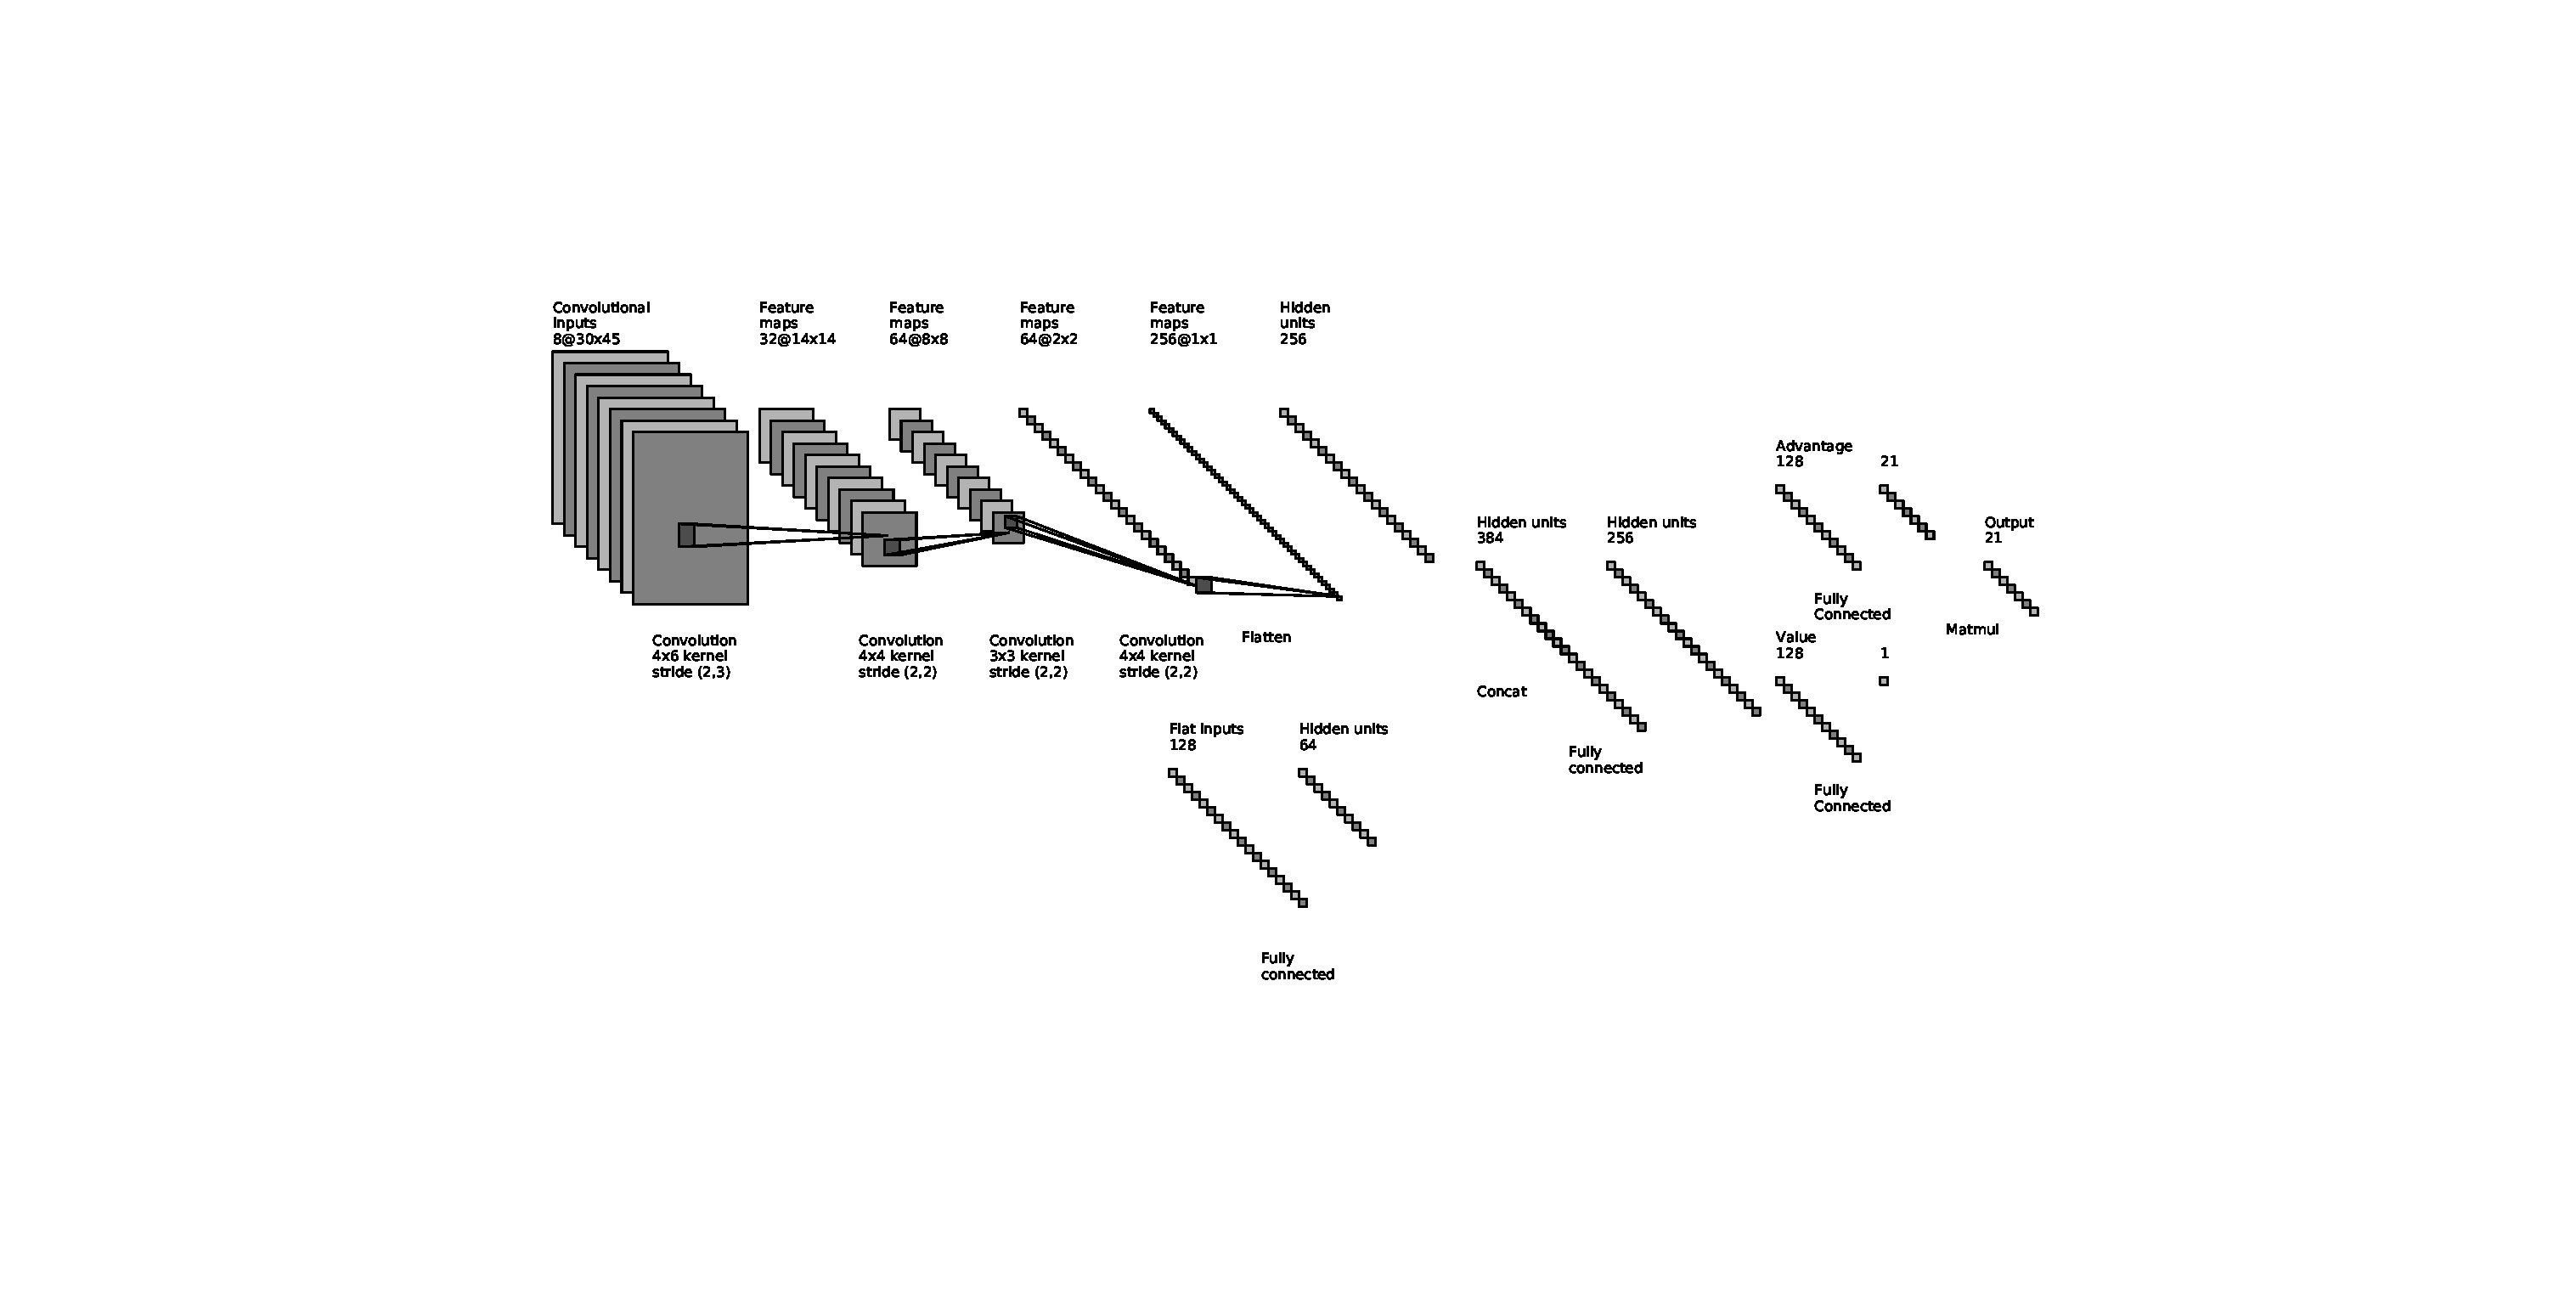
\includegraphics[trim={10cm 6cm 10cm 5.5cm},clip,width=\textwidth]{DQN_structure}
	\caption{The used convolutional DQN-network with a dueling architecture}
	\label{fig:dqn_graph}
\end{figure}

In a hybrid ANN (having both 2D and 1D input), four convolutional layers calculate an abstract representation of the two-dimensional inputs, which is flattened into a hidden layer consisting of 256 Units. The one-dimensional input are connected via a dense layer to another hidden layer of 64 units. These two layers are then concatenated to form a layer of 384 hidden Units, which is densely connected to a furhter hidden layer, which splits into an advantage and a value stream as proposed by \cite{wang_dueling_2015}. While the advantage stream ends in a layer with one unit for each action, the value-stream has one output. In the very last layer of the network, the advantage and value stream are combined into the final output layer, providing a separate Q-value for each action.



1. dqn-algorithm
- anzahl layer, Batchnorm, doubles dueling
- clipping wieder rein, reference auf das dueling
- grundsätzlich gegen batchnorm entschieden, siehe reddit post
- MIT GRAFIK
- Adam und tensorflow quoten, siehe zotero
2. ddpg
- anzahl layer, Batchnorm
- MIT GRAFIK

-mo
-schöne grafik.
-auf meien DQN-config eingehen und(!!!) ne DDPG-config machen, using the "experiment details" vom ddpg paper  


In the original DDPG-algorithm \cite{lillicrap_continuous_2015}, the authors used \keyword{batch normalization} \cite{ioffe_batch_2015} to have the possibility of using the same network hyperparameters for differently scaled input-values. In the learning step when using minibatches, \batchnorm normalizes each dimension across the samples in a batch to have unit mean and variance, whilst keeping a running mean and variance to normalize in non-learning steps. In Tensorflow, batchnorm can be added with an additional layer and an additional input, specifying the phase (learning step/non-learning step)\footnote{cf. \url{https://www.tensorflow.org/api\_docs/python/tf/contrib/layers/batch_norm}}. Though Lillicrap et al. seemed to have success on using \batchnorm, in practice it lead to unstability, even on simple physics tasks in openAI's gym. As I am not the only one having this issue \footnote{redditlink}, I left out batch normalization for good.





\paragraph{DDPG}

-die grafik von andrea
-satz über batchnorm




%[dass die alle plotter HABEN und die serverkompomenten über containers KENNen etc]... doch nochmal in nem großem uml-diagram? dann auch als notiz rein dass bei nem actual agent der gameState weg-abstrahiert ist ... und inklusive agent has evaluator, evaluator knows agent, ... same for memory, ...

%[die architektur von meinem duelDQN muss nochmal inen eigenen graphen yay]

%%-alle FOREVERYINF schritte führt der agent dann COMESALEARN learn-schritte durch (definiert in der dauerLearnANN/learnANN des agents.py, welche wiederum q_learn von ddddqn.py callen)
%
%Was der Fehler sooooo lange war: Das Auto fährt immer direkt gegen die Wand. Im laufe der Exploration fährt es halt anfangs ein bisschen random, unter anderem den schnellsten weg an die Wand (1, 0, 0.875). Nach dem trianing denkt es sich dann hey, schnellster weg gegen die wand, perfekt, genau das will ich. Hat durchgehend den höchsten Q-wert, vom losfahren bis direkt vor der wand stehen.
%
%
%State    action    reward  state2  is_terminal
%0.253   (1, 0, 0.857)   1.085   1.052   False
%1.052   (1, 0, 0.857)   1.07488 1.965   False
%1.965   (1, 0, 0.857)   1.06112 2.989   False
%2.989   (1, 0, 0.857)   1.0428   4.118   False
%4.118   (1, 0, 0.857)   0   5.334   False
%5.334   (1, 0, 0.857)   0   6.626   False
%6.626   (1, 0, 0.857)   0   7.955   False
%7.955   (1, 0, 0.857)   0   9.322   False
%9.322   (1, 0, 0.857)   0   10.0  False
%10.0   (0, 0, 0.857)   -5   10.0   True




%
%[tf gibt automatic differentiation, multi-gpu support, python interface]
%


%mehr pseudocodes!!!!




% TODO \subsubsection{Challenges and Solutions}

% TODO \subsection{Performance measure}

% TODO dden -help command-line parameter erwähnen
% TODO -dass halt eigentlich zu jedem zeitpunkt compared zu rrt oder human sein müsste

\section{Possible features}

\label{ch:possiblefeatures}

\subsection{The vectors}

\label{ch:thevectors}

%-progressvec (progress, laptime, lapcount, validvec)
%-speedsteer (motortorques, steerangle, velocity, fRightDirection, velocity of perpendiculars, angle, speedinstreetdir, speedintraversedir, cuvinessbeforecar)
%-carstatusvec (longitutinal and latidutialn slip for each tire)
%-centerdist, als vector
%-waldistvec (direction the car faces, steers, moves..... and directiont the street goes (each longsighted and shortsighted from car and streetmiddle)
%-lookahead-vector
%-delta und feedback
%-actual action (possibly overwritten)
%-both vision-vectors

\term{Possible Vectors} refers to all information the game streams over its socket to the agent. While most of this information will be used to make up an agent's state, the vectors also provide information about if the game must be reset as well as information to calculate the reward from. This information is collected in Unity in the function \codefunc{GetAllInfos()}, and converted into a namedtuple-wrapper called \codeobj{Otherinputs}, specified in \filename{read\_supervised.py}. In this section, I provide an overview of those vectors and their meaning in the game. I refer to the individual possible vectors by the name used in \codeobj{Otherinputs}.

\paragraph{ProgressVec} This vector contains information about the current progress of the car on the track, which consists of the actual progress in percent, the time the car needed for the current lap so far, the number of the current lap, as well as the flag if the round is still valid (which is the case if the car did not leave the street yet).

\paragraph{SpeedSteer} In this vector, information about the car's velocity and its steer angle is encoded. It consists of the following values:

\renewcommand{\arraystretch}{1.3}
\begin{flushleft}
\begin{tabular}{>{\em}p{2.9cm} p{\textwidth-3.8cm}} 
	RLTorque & The motor torque applied to the left back tire\\
	RRTorque & The motor torque applied to the right back tire\\
	FLSteer & The steering angle of the front left tire\\
	FRSteer & The steering angle of the front right tire\\
	velocity & The velocity of the car as scalar independent of directions\\
	rightDirection & A boolean value if the car moves into the intended direction\\
	velocityOfPerpendiculars & \hspace*{0.8cm} The velocity of the orthogonal projection of the car onto the center of the street\\ %TODO see sectionbalabla, wo ich DOCH die definition von perpendicular einführen werde
	carAngle & The car's angle (in degrees) in relation to the street's direction\\
	speedInStreetDir & The car's velocity into the street's direction (calculated using the dot-product between the car's velocity-vectors and the direction-vector of the street at the car's current position)\\
	speedInTraverDir &  The car's velocity into the orthogonal of the street's direction\\
	CurvinessBeforeCar & A measure of the curvature of the street immediately ahead of the car ($CurvinessBeforeCar \in [0,1]$, where a value of zero corresponds to a straight street)\\	
\end{tabular}
\end{flushleft}

\paragraph{StatusVector} This vector contains eight values, corresponding to the forward slip and sideways slip of each of the car's tires, using a function provided for Unity's \codeobj{WheelCollider}-object. The more the car slips, the smaller the impact of movement commands. The current slip-values are presented in the GUI of the game (and can be seen behind annotation \textbf{R} in figure~\ref{fig:aidriveshot}).

\paragraph{CenterDist and CenterDistVec} The \emph{CenterDist} corresponds to the car's orthogonal center to the street's center, as calculated in \colorbox{red}{where} (also visually represented in the car's GUI, behind annotation \textbf{N} in figure~\ref{fig:aidriveshot}).
The \emph{CenterDistVec} contains the same information presented in another way: It is a vector of length 15, where the middle element corresponds to the car's longitutional position. The other elemnts correspond to points with regular distances to the car's left and right. The value of each respective element is calculated using the reversed distance between this position and the longitudional center of the street. The content of this vector is visually represented behind annotation \textbf{M} in figure~\ref{fig:aidriveshot}.

\paragraph{WallDistVec} This vector contains seven values, corresponding to the car's distance to the wall along a certain ray. It does not contain the closest distance to the wall -- because this value is already represented by the CenterDist. As the wall has always a fixed distance from the street's center (with an absolute value of five), the distance to the closest wall can be calculated as $5 - abs(CenterDist)$. 
For the calculation of the \emph{WallDistVec}, several rays are casted from the car's (or the perpendicular's) position into a particular direction. Returned is then the distance from their respective origin and their first intersection with a wall. The vector contains seven values, using rays with different origins and different directions. In the following table, I provide an explanation of each of those values, while figure~\ref{fig:walldistvec} in appendix~\ref{AppendixB} visually represents these rays. The respective color is mentioned in the table.
\renewcommand{\arraystretch}{1.3}
\begin{flushleft}
	\begin{tabular}{p{0.5cm} p{2cm} p{2.4cm} p{\textwidth-6.45cm}} 
		\# & color in \ref{fig:walldistvec} & origin & direction \\
		\hline
		1 & \textcolor{black}{black} & car's center & direction the car faces \\
		2 & \textcolor{magenta}{magenta} & car's center & direction the car steers\\	
		3 & \textcolor{red}{red} & car's center & direction the car moves\\	
		4 & \textcolor{black}{white} & car's center & short-sighted direction of the street (calculated as the vector between the closest \codeobj{anchorVector} behind the car and the closest one before the car) \\		
		5 & \textcolor{yellow}{yellow} & perpendicular & short-sighted direction of the street (calculated as the vector between the closest \codeobj{anchorVector} behind the car and the closest one before the car) \\
		6 & \textcolor{blue}{blue} & car's center & long-sighted direction of the street (calculated as the vector between the closest \codeobj{anchorVector}  to the car and the one 5 in advance) \\
		7 & \textcolor{gray}{gray} & perpendicular & long-sighted direction of the street (calculated as the vector between the closest \codeobj{anchorVector}  to the car and the one 5 in advance) \\
	\end{tabular}
\end{flushleft}

\paragraph{LookAheadVec} This vector corresponds to the course of the street ahead of the car. It is a vector consisting of 30 elements, corresponding to regularly spaced \codeobj{anchorVector}s, starting at the position of the car, following the direction of the street. The value at each position $i$ of this vector corresponds to the angle between the direction of the street at position $i$ and the direction at position $i+1$. In other words, if the street makes a shart turn 4 units ahead of the car, then element $3$ will contain a high value. The angle is measured in degrees. A graphical representation of this vector can be seen behind annotation \textbf{N} in figure~\ref{fig:aidriveshot}.

\paragraph{FBDelta} This vector consists of two values, namely \emph{Feedback} and \empf{Delta}. The Feedback-value is the temporal difference of how long the car needed for a specific section of the course (constrained via the closest \codeobj{anchorVector}s of the car) in the current process in comparison to the time needed in the fastest lap so far. The Delta-value is the absolute difference in time needed for the entire lap so far.

As both of these values are only useful in relation to the time needed for the fastest lap, it must be ensured that this does not change during training. For that, The file \filename{AiInterface.cs} contains in its class \codeobj{Consts} a flag \codeobj{lock\_fastestlap\_in\_AIMode}. Note however, that even if this flag is set, the values of \emph{FBDelta} could at most be used to calculate the agent's reward and not as part of its state.

\paragraph{Action} This is a three-dimensional vector corresponding to the actual action the environment recorded. While the agent knows what action it provided, it could be manually overwritten (after the press of \keystroke{H}) -- which is why the agent stores this vector in its replay memory instead of the action it would have performed otherwise.


\paragraph{Mini-maps} While the content of the mini-maps is not contained in the namedtuple \codeobj{Otherinput}, their value is transmitted from the game just like the other vectors. In the current implementation, both cameras have a resolution of $30\times45$ pixels, where one camera is $15$ units away of the car, and the other one $75$ units, which means that the former provides a smaller but more detailed view of the car. The closer camera is mostly referred to as $vvec2$, whereas the other one is denoted $visionvec$ or $vvec$.\\

As a working game was already provided by \leon of this thesis, so where some of these vectors, namely the calculation of FBDelta, LookAheadVec, CenterDist and CenterDistVec, as well as many elements necessary to compute many of the other ones.

\subsection{Exploration}

Only very basic exploration algorithms are provided in this thesis. There are two different methods used in the DQN-based agents compared to the agents with a DDPG-model, following their definition of an action. While in DDPG-based agents it holds that $action \subset \mathds{R}^{n \in \mathds{N}}$, in DQN-based agent the action is discretized into one unique value. 

While the action-value 

-epsilon-greedy als standard und make_noisy vom DDPG

\subsection{Reward}

-meine theorien: continuous, non-negative, aus ner shclehcten darf nicht besser sein als in einem guten eh sein)
-dass immer speed belohnen negativ ist, siehe ->problem bei ddpg, approach von dem kerastorcsguy, siehe kapitel \colorbox{red}{Daskapitel}
-die funktion wo man sich den durchgängingen reward in ner farbe plotten kann (auch bei \keystroke{H})

